\documentclass[twoside]{book}

% Packages required by doxygen
\usepackage{calc}
\usepackage{doxygen}
\usepackage{graphicx}
\usepackage[utf8]{inputenc}
\usepackage{makeidx}
\usepackage{multicol}
\usepackage{multirow}
\usepackage{textcomp}
\usepackage[table]{xcolor}

% Font selection
\usepackage[T1]{fontenc}
\usepackage{mathptmx}
\usepackage[scaled=.90]{helvet}
\usepackage{courier}
\usepackage{amssymb}
\usepackage{sectsty}
\renewcommand{\familydefault}{\sfdefault}
\allsectionsfont{%
  \fontseries{bc}\selectfont%
  \color{darkgray}%
}
\renewcommand{\DoxyLabelFont}{%
  \fontseries{bc}\selectfont%
  \color{darkgray}%
}

% Page & text layout
\usepackage{geometry}
\geometry{%
  a4paper,%
  top=2.5cm,%
  bottom=2.5cm,%
  left=2.5cm,%
  right=2.5cm%
}
\tolerance=750
\hfuzz=15pt
\hbadness=750
\setlength{\emergencystretch}{15pt}
\setlength{\parindent}{0cm}
\setlength{\parskip}{0.2cm}
\makeatletter
\renewcommand{\paragraph}{%
  \@startsection{paragraph}{4}{0ex}{-1.0ex}{1.0ex}{%
    \normalfont\normalsize\bfseries\SS@parafont%
  }%
}
\renewcommand{\subparagraph}{%
  \@startsection{subparagraph}{5}{0ex}{-1.0ex}{1.0ex}{%
    \normalfont\normalsize\bfseries\SS@subparafont%
  }%
}
\makeatother

% Headers & footers
\usepackage{fancyhdr}
\pagestyle{fancyplain}
\fancyhead[LE]{\fancyplain{}{\bfseries\thepage}}
\fancyhead[CE]{\fancyplain{}{}}
\fancyhead[RE]{\fancyplain{}{\bfseries\leftmark}}
\fancyhead[LO]{\fancyplain{}{\bfseries\rightmark}}
\fancyhead[CO]{\fancyplain{}{}}
\fancyhead[RO]{\fancyplain{}{\bfseries\thepage}}
\fancyfoot[LE]{\fancyplain{}{}}
\fancyfoot[CE]{\fancyplain{}{}}
\fancyfoot[RE]{\fancyplain{}{\bfseries\scriptsize Generated on Thu Oct 30 2014 15\-:04\-:36 for digiholo2\-D by Doxygen }}
\fancyfoot[LO]{\fancyplain{}{\bfseries\scriptsize Generated on Thu Oct 30 2014 15\-:04\-:36 for digiholo2\-D by Doxygen }}
\fancyfoot[CO]{\fancyplain{}{}}
\fancyfoot[RO]{\fancyplain{}{}}
\renewcommand{\footrulewidth}{0.4pt}
\renewcommand{\chaptermark}[1]{%
  \markboth{#1}{}%
}
\renewcommand{\sectionmark}[1]{%
  \markright{\thesection\ #1}%
}

% Indices & bibliography
\usepackage{natbib}
\usepackage[titles]{tocloft}
\setcounter{tocdepth}{3}
\setcounter{secnumdepth}{5}
\makeindex

% Hyperlinks (required, but should be loaded last)
\usepackage{ifpdf}
\ifpdf
  \usepackage[pdftex,pagebackref=true]{hyperref}
\else
  \usepackage[ps2pdf,pagebackref=true]{hyperref}
\fi
\hypersetup{%
  colorlinks=true,%
  linkcolor=blue,%
  citecolor=blue,%
  unicode%
}

% Custom commands
\newcommand{\clearemptydoublepage}{%
  \newpage{\pagestyle{empty}\cleardoublepage}%
}


%===== C O N T E N T S =====

\begin{document}

% Titlepage & ToC
\hypersetup{pageanchor=false}
\pagenumbering{roman}
\begin{titlepage}
\vspace*{7cm}
\begin{center}%
{\Large digiholo2\-D }\\
\vspace*{1cm}
{\large Generated by Doxygen 1.8.6}\\
\vspace*{0.5cm}
{\small Thu Oct 30 2014 15:04:36}\\
\end{center}
\end{titlepage}
\clearemptydoublepage
\tableofcontents
\clearemptydoublepage
\pagenumbering{arabic}
\hypersetup{pageanchor=true}

%--- Begin generated contents ---
\chapter{Hierarchical Index}
\section{Class Hierarchy}
This inheritance list is sorted roughly, but not completely, alphabetically\-:\begin{DoxyCompactList}
\item \contentsline{section}{abstract\-\_\-fringe\-\_\-analyser}{\pageref{classabstract__fringe__analyser}}{}
\begin{DoxyCompactList}
\item \contentsline{section}{Takeda\-\_\-\-F\-F\-T\-W\-\_\-fringe\-\_\-analyser}{\pageref{class_takeda___f_f_t_w__fringe__analyser}}{}
\end{DoxyCompactList}
\item \contentsline{section}{abstract\-\_\-smart\-\_\-tile\-\_\-unwrapper}{\pageref{classabstract__smart__tile__unwrapper}}{}
\item \contentsline{section}{abstract\-\_\-smart\-\_\-unwrapper}{\pageref{classabstract__smart__unwrapper}}{}
\item \contentsline{section}{abstract\-\_\-tile\-\_\-merger}{\pageref{classabstract__tile__merger}}{}
\begin{DoxyCompactList}
\item \contentsline{section}{simple1d\-\_\-tile\-\_\-merger}{\pageref{classsimple1d__tile__merger}}{}
\item \contentsline{section}{srncp\-\_\-tile\-\_\-merger}{\pageref{classsrncp__tile__merger}}{}
\end{DoxyCompactList}
\item \contentsline{section}{abstract\-\_\-tile\-\_\-unwrapper}{\pageref{classabstract__tile__unwrapper}}{}
\begin{DoxyCompactList}
\item \contentsline{section}{grad\-\_\-fit\-\_\-tile\-\_\-unwrapper}{\pageref{classgrad__fit__tile__unwrapper}}{}
\item \contentsline{section}{minimization\-\_\-tile\-\_\-unwrapper}{\pageref{classminimization__tile__unwrapper}}{}
\item \contentsline{section}{Strand\-\_\-tile\-\_\-unwrapper}{\pageref{class_strand__tile__unwrapper}}{}
\end{DoxyCompactList}
\item \contentsline{section}{abstract\-\_\-unwrapper}{\pageref{classabstract__unwrapper}}{}
\begin{DoxyCompactList}
\item \contentsline{section}{srncp\-\_\-unwrapper}{\pageref{classsrncp__unwrapper}}{}
\item \contentsline{section}{tile\-\_\-merge\-\_\-unwrapper}{\pageref{classtile__merge__unwrapper}}{}
\end{DoxyCompactList}
\item \contentsline{section}{E\-D\-G\-E}{\pageref{struct_e_d_g_e}}{}
\item \contentsline{section}{float\-\_\-image}{\pageref{classfloat__image}}{}
\begin{DoxyCompactList}
\item \contentsline{section}{col\-\_\-major\-\_\-float\-\_\-image}{\pageref{classcol__major__float__image}}{}
\item \contentsline{section}{row\-\_\-major\-\_\-float\-\_\-image}{\pageref{classrow__major__float__image}}{}
\end{DoxyCompactList}
\item \contentsline{section}{P\-I\-X\-E\-L}{\pageref{struct_p_i_x_e_l}}{}
\item Q\-Main\-Window\begin{DoxyCompactList}
\item \contentsline{section}{digiholo\-Main\-Gui}{\pageref{classdigiholo_main_gui}}{}
\end{DoxyCompactList}
\item \contentsline{section}{qt\-\_\-meta\-\_\-stringdata\-\_\-digiholo\-Main\-Gui\-\_\-t}{\pageref{structqt__meta__stringdata__digiholo_main_gui__t}}{}
\item \contentsline{section}{qt\-\_\-meta\-\_\-stringdata\-\_\-\-Reconstruction\-Thread\-\_\-t}{\pageref{structqt__meta__stringdata___reconstruction_thread__t}}{}
\item Q\-Thread\begin{DoxyCompactList}
\item \contentsline{section}{Reconstruction\-Thread}{\pageref{class_reconstruction_thread}}{}
\end{DoxyCompactList}
\item \contentsline{section}{smart\-\_\-tile}{\pageref{classsmart__tile}}{}
\item \contentsline{section}{smart\-\_\-tile\-\_\-junction}{\pageref{classsmart__tile__junction}}{}
\item \contentsline{section}{smart\-\_\-tiled\-\_\-image}{\pageref{classsmart__tiled__image}}{}
\item \contentsline{section}{smart\-\_\-tilegroup}{\pageref{classsmart__tilegroup}}{}
\item \contentsline{section}{tesselated\-\_\-image}{\pageref{classtesselated__image}}{}
\item \contentsline{section}{tile}{\pageref{classtile}}{}
\item \contentsline{section}{tile\-\_\-image}{\pageref{classtile__image}}{}
\item \contentsline{section}{tile\-\_\-junction}{\pageref{classtile__junction}}{}
\item \contentsline{section}{tilegroup}{\pageref{classtilegroup}}{}
\item \contentsline{section}{Ui\-\_\-digiholo\-Main\-Gui}{\pageref{class_ui__digiholo_main_gui}}{}
\begin{DoxyCompactList}
\item \contentsline{section}{Ui\-:\-:digiholo\-Main\-Gui}{\pageref{class_ui_1_1digiholo_main_gui}}{}
\end{DoxyCompactList}
\end{DoxyCompactList}

\chapter{Class Index}
\section{Class List}
Here are the classes, structs, unions and interfaces with brief descriptions\-:\begin{DoxyCompactList}
\item\contentsline{section}{\hyperlink{classabstract__fringe__analyser}{abstract\-\_\-fringe\-\_\-analyser} }{\pageref{classabstract__fringe__analyser}}{}
\item\contentsline{section}{\hyperlink{classabstract__smart__tile__unwrapper}{abstract\-\_\-smart\-\_\-tile\-\_\-unwrapper} }{\pageref{classabstract__smart__tile__unwrapper}}{}
\item\contentsline{section}{\hyperlink{classabstract__smart__unwrapper}{abstract\-\_\-smart\-\_\-unwrapper} }{\pageref{classabstract__smart__unwrapper}}{}
\item\contentsline{section}{\hyperlink{classabstract__tile__merger}{abstract\-\_\-tile\-\_\-merger} }{\pageref{classabstract__tile__merger}}{}
\item\contentsline{section}{\hyperlink{classabstract__tile__unwrapper}{abstract\-\_\-tile\-\_\-unwrapper} }{\pageref{classabstract__tile__unwrapper}}{}
\item\contentsline{section}{\hyperlink{classabstract__unwrapper}{abstract\-\_\-unwrapper} }{\pageref{classabstract__unwrapper}}{}
\item\contentsline{section}{\hyperlink{classcol__major__float__image}{col\-\_\-major\-\_\-float\-\_\-image} }{\pageref{classcol__major__float__image}}{}
\item\contentsline{section}{\hyperlink{class_ui_1_1digiholo_main_gui}{Ui\-::digiholo\-Main\-Gui} }{\pageref{class_ui_1_1digiholo_main_gui}}{}
\item\contentsline{section}{\hyperlink{classdigiholo_main_gui}{digiholo\-Main\-Gui} }{\pageref{classdigiholo_main_gui}}{}
\item\contentsline{section}{\hyperlink{struct_e_d_g_e}{E\-D\-G\-E} }{\pageref{struct_e_d_g_e}}{}
\item\contentsline{section}{\hyperlink{classfloat__image}{float\-\_\-image} }{\pageref{classfloat__image}}{}
\item\contentsline{section}{\hyperlink{classgrad__fit__tile__unwrapper}{grad\-\_\-fit\-\_\-tile\-\_\-unwrapper} }{\pageref{classgrad__fit__tile__unwrapper}}{}
\item\contentsline{section}{\hyperlink{classminimization__tile__unwrapper}{minimization\-\_\-tile\-\_\-unwrapper} }{\pageref{classminimization__tile__unwrapper}}{}
\item\contentsline{section}{\hyperlink{struct_p_i_x_e_l}{P\-I\-X\-E\-L} }{\pageref{struct_p_i_x_e_l}}{}
\item\contentsline{section}{\hyperlink{structqt__meta__stringdata__digiholo_main_gui__t}{qt\-\_\-meta\-\_\-stringdata\-\_\-digiholo\-Main\-Gui\-\_\-t} }{\pageref{structqt__meta__stringdata__digiholo_main_gui__t}}{}
\item\contentsline{section}{\hyperlink{structqt__meta__stringdata___reconstruction_thread__t}{qt\-\_\-meta\-\_\-stringdata\-\_\-\-Reconstruction\-Thread\-\_\-t} }{\pageref{structqt__meta__stringdata___reconstruction_thread__t}}{}
\item\contentsline{section}{\hyperlink{class_reconstruction_thread}{Reconstruction\-Thread} }{\pageref{class_reconstruction_thread}}{}
\item\contentsline{section}{\hyperlink{classrow__major__float__image}{row\-\_\-major\-\_\-float\-\_\-image} }{\pageref{classrow__major__float__image}}{}
\item\contentsline{section}{\hyperlink{classsimple1d__tile__merger}{simple1d\-\_\-tile\-\_\-merger} }{\pageref{classsimple1d__tile__merger}}{}
\item\contentsline{section}{\hyperlink{classsmart__tile}{smart\-\_\-tile} }{\pageref{classsmart__tile}}{}
\item\contentsline{section}{\hyperlink{classsmart__tile__junction}{smart\-\_\-tile\-\_\-junction} }{\pageref{classsmart__tile__junction}}{}
\item\contentsline{section}{\hyperlink{classsmart__tiled__image}{smart\-\_\-tiled\-\_\-image} }{\pageref{classsmart__tiled__image}}{}
\item\contentsline{section}{\hyperlink{classsmart__tilegroup}{smart\-\_\-tilegroup} }{\pageref{classsmart__tilegroup}}{}
\item\contentsline{section}{\hyperlink{classsrncp__tile__merger}{srncp\-\_\-tile\-\_\-merger} }{\pageref{classsrncp__tile__merger}}{}
\item\contentsline{section}{\hyperlink{classsrncp__unwrapper}{srncp\-\_\-unwrapper} }{\pageref{classsrncp__unwrapper}}{}
\item\contentsline{section}{\hyperlink{class_strand__tile__unwrapper}{Strand\-\_\-tile\-\_\-unwrapper} }{\pageref{class_strand__tile__unwrapper}}{}
\item\contentsline{section}{\hyperlink{class_takeda___f_f_t_w__fringe__analyser}{Takeda\-\_\-\-F\-F\-T\-W\-\_\-fringe\-\_\-analyser} }{\pageref{class_takeda___f_f_t_w__fringe__analyser}}{}
\item\contentsline{section}{\hyperlink{classtesselated__image}{tesselated\-\_\-image} }{\pageref{classtesselated__image}}{}
\item\contentsline{section}{\hyperlink{classtile}{tile} }{\pageref{classtile}}{}
\item\contentsline{section}{\hyperlink{classtile__image}{tile\-\_\-image} }{\pageref{classtile__image}}{}
\item\contentsline{section}{\hyperlink{classtile__junction}{tile\-\_\-junction} }{\pageref{classtile__junction}}{}
\item\contentsline{section}{\hyperlink{classtile__merge__unwrapper}{tile\-\_\-merge\-\_\-unwrapper} }{\pageref{classtile__merge__unwrapper}}{}
\item\contentsline{section}{\hyperlink{classtilegroup}{tilegroup} }{\pageref{classtilegroup}}{}
\item\contentsline{section}{\hyperlink{class_ui__digiholo_main_gui}{Ui\-\_\-digiholo\-Main\-Gui} }{\pageref{class_ui__digiholo_main_gui}}{}
\end{DoxyCompactList}

\chapter{Class Documentation}
\hypertarget{classabstract__fringe__analyser}{\section{abstract\-\_\-fringe\-\_\-analyser Class Reference}
\label{classabstract__fringe__analyser}\index{abstract\-\_\-fringe\-\_\-analyser@{abstract\-\_\-fringe\-\_\-analyser}}
}
Inheritance diagram for abstract\-\_\-fringe\-\_\-analyser\-:\begin{figure}[H]
\begin{center}
\leavevmode
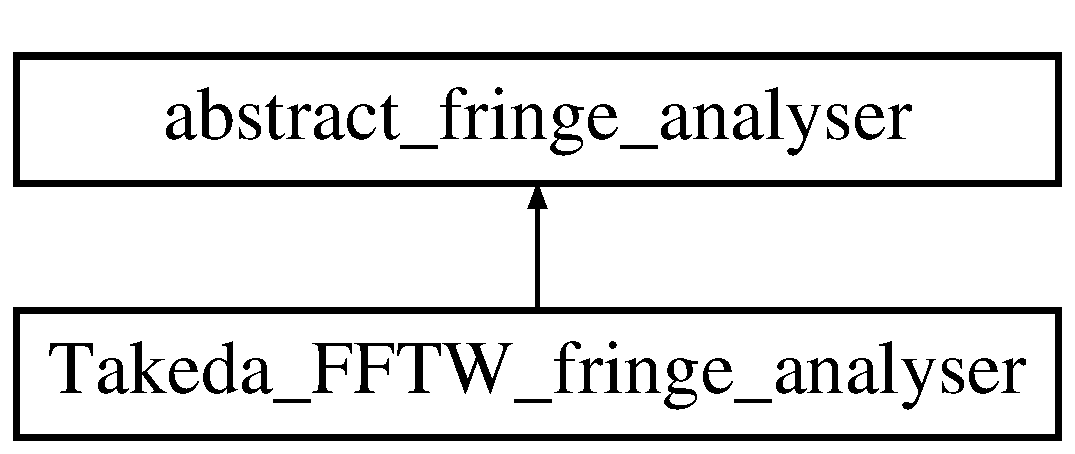
\includegraphics[height=2.000000cm]{classabstract__fringe__analyser}
\end{center}
\end{figure}
\subsection*{Public Member Functions}
\begin{DoxyCompactItemize}
\item 
virtual bool \hyperlink{classabstract__fringe__analyser_a48f796b6b3d8dbf9dd66f5e5eaf98153}{calc\-\_\-wrapped\-\_\-phase\-\_\-map} (\hyperlink{classfloat__image}{float\-\_\-image} $\ast$fringe\-\_\-pattern, \hyperlink{classfloat__image}{float\-\_\-image} $\ast$wrapped\-\_\-phase\-\_\-map)=0
\end{DoxyCompactItemize}


\subsection{Detailed Description}
abstrahiert die Funktionalität aus einem Interferenzbild die (gewrappte!) Phase zu berechnen. Abgeleiteten Klassen sollen alle nötigen Parameter im Konstruktor übergeben werden. 

\subsection{Member Function Documentation}
\hypertarget{classabstract__fringe__analyser_a48f796b6b3d8dbf9dd66f5e5eaf98153}{\index{abstract\-\_\-fringe\-\_\-analyser@{abstract\-\_\-fringe\-\_\-analyser}!calc\-\_\-wrapped\-\_\-phase\-\_\-map@{calc\-\_\-wrapped\-\_\-phase\-\_\-map}}
\index{calc\-\_\-wrapped\-\_\-phase\-\_\-map@{calc\-\_\-wrapped\-\_\-phase\-\_\-map}!abstract_fringe_analyser@{abstract\-\_\-fringe\-\_\-analyser}}
\subsubsection[{calc\-\_\-wrapped\-\_\-phase\-\_\-map}]{\setlength{\rightskip}{0pt plus 5cm}virtual bool abstract\-\_\-fringe\-\_\-analyser\-::calc\-\_\-wrapped\-\_\-phase\-\_\-map (
\begin{DoxyParamCaption}
\item[{{\bf float\-\_\-image} $\ast$}]{fringe\-\_\-pattern, }
\item[{{\bf float\-\_\-image} $\ast$}]{wrapped\-\_\-phase\-\_\-map}
\end{DoxyParamCaption}
)\hspace{0.3cm}{\ttfamily [pure virtual]}}}\label{classabstract__fringe__analyser_a48f796b6b3d8dbf9dd66f5e5eaf98153}
Berechnet eine wrapped Phase map aus einem Fringe Image aus float Daten. 
\begin{DoxyParams}{Parameters}
{\em fringe\-\_\-pattern} & Das Interferenzbild. \\
\hline
{\em wrapped\-\_\-phase\-\_\-map} & Pointer mit Platz für die berechnete wrapped phase map. \\
\hline
\end{DoxyParams}
\begin{DoxyReturn}{Returns}
true if everything went well, false if not 
\end{DoxyReturn}


Implemented in \hyperlink{class_takeda___f_f_t_w__fringe__analyser_a0213cf26993557bf87b5c14d8b354582}{Takeda\-\_\-\-F\-F\-T\-W\-\_\-fringe\-\_\-analyser}.



The documentation for this class was generated from the following file\-:\begin{DoxyCompactItemize}
\item 
include/abstract\-\_\-fringe\-\_\-analyser.\-h\end{DoxyCompactItemize}

\input{classabstract__smart__tile__unwrapper}
\input{classabstract__smart__unwrapper}
\hypertarget{classabstract__tile__merger}{\section{abstract\-\_\-tile\-\_\-merger Class Reference}
\label{classabstract__tile__merger}\index{abstract\-\_\-tile\-\_\-merger@{abstract\-\_\-tile\-\_\-merger}}
}
Inheritance diagram for abstract\-\_\-tile\-\_\-merger\-:\begin{figure}[H]
\begin{center}
\leavevmode
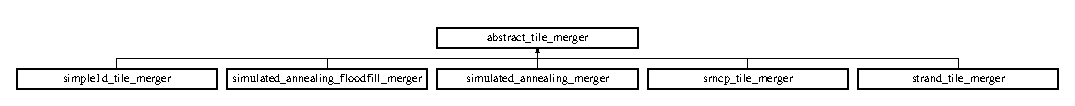
\includegraphics[height=2.000000cm]{classabstract__tile__merger}
\end{center}
\end{figure}
\subsection*{Public Member Functions}
\begin{DoxyCompactItemize}
\item 
virtual void \hyperlink{classabstract__tile__merger_a60e28617e046734ef14ce15704a79680}{merge\-\_\-tiles} (\hyperlink{classtesselated__image}{tesselated\-\_\-image} $\ast$t)=0
\end{DoxyCompactItemize}


\subsection{Detailed Description}
provides the abstract interface for merging unwrapped tiles to a single unwrapped phase image. 

\subsection{Member Function Documentation}
\hypertarget{classabstract__tile__merger_a60e28617e046734ef14ce15704a79680}{\index{abstract\-\_\-tile\-\_\-merger@{abstract\-\_\-tile\-\_\-merger}!merge\-\_\-tiles@{merge\-\_\-tiles}}
\index{merge\-\_\-tiles@{merge\-\_\-tiles}!abstract_tile_merger@{abstract\-\_\-tile\-\_\-merger}}
\subsubsection[{merge\-\_\-tiles}]{\setlength{\rightskip}{0pt plus 5cm}virtual void abstract\-\_\-tile\-\_\-merger\-::merge\-\_\-tiles (
\begin{DoxyParamCaption}
\item[{{\bf tesselated\-\_\-image} $\ast$}]{t}
\end{DoxyParamCaption}
)\hspace{0.3cm}{\ttfamily [pure virtual]}}}\label{classabstract__tile__merger_a60e28617e046734ef14ce15704a79680}
This method merges tiles from a tesselated wrapped phase image to an unwrapped image. These tiles alreasy need to be unwrapped individually and are then unwrapped with respect to each other to form an unwrapped phase map. 

Implemented in \hyperlink{classsrncp__tile__merger_a8513af3c4d4dd03ef9b50973edafb01b}{srncp\-\_\-tile\-\_\-merger}, and \hyperlink{classsimple1d__tile__merger_a33c12f0c71ad8d05a4644d027060a17b}{simple1d\-\_\-tile\-\_\-merger}.



The documentation for this class was generated from the following file\-:\begin{DoxyCompactItemize}
\item 
include/block\-\_\-srncp/abstract\-\_\-tile\-\_\-merger.\-h\end{DoxyCompactItemize}

\hypertarget{classabstract__tile__unwrapper}{\section{abstract\-\_\-tile\-\_\-unwrapper Class Reference}
\label{classabstract__tile__unwrapper}\index{abstract\-\_\-tile\-\_\-unwrapper@{abstract\-\_\-tile\-\_\-unwrapper}}
}


{\ttfamily \#include $<$abstract\-\_\-tile\-\_\-unwrapper.\-h$>$}

Inheritance diagram for abstract\-\_\-tile\-\_\-unwrapper\-:\begin{figure}[H]
\begin{center}
\leavevmode
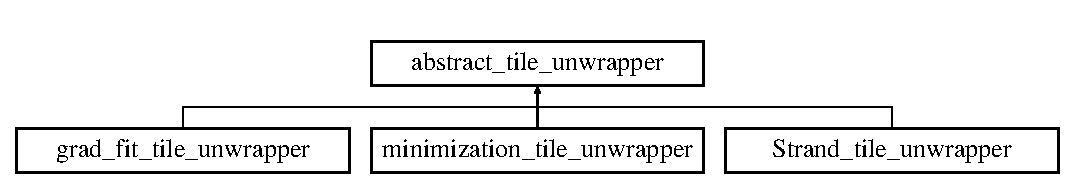
\includegraphics[height=1.885522cm]{classabstract__tile__unwrapper}
\end{center}
\end{figure}
\subsection*{Public Member Functions}
\begin{DoxyCompactItemize}
\item 
\hyperlink{classabstract__tile__unwrapper_a31fc3a41d4adaab0ba7c2998e74ccedb}{abstract\-\_\-tile\-\_\-unwrapper} ()
\item 
virtual void \hyperlink{classabstract__tile__unwrapper_a74eedd36e55b9000b5986ff5980a563a}{unwrap} (boost\-::shared\-\_\-ptr$<$ \hyperlink{classtile}{tile} $>$ t)=0
\item 
virtual std\-::string \hyperlink{classabstract__tile__unwrapper_ae70f69a703e622e5ab13eabcc91fca4d}{get\-\_\-name} ()=0
\item 
virtual void \hyperlink{classabstract__tile__unwrapper_a469b36a7f302d5a2655631bbdb6f8daf}{usage\-\_\-help} ()=0
\end{DoxyCompactItemize}


\subsection{Detailed Description}
This pure virtual class provides an abstract interface for an unwrapper that unwraps a single tile. It operates with boost smart pointers. 

\subsection{Constructor \& Destructor Documentation}
\hypertarget{classabstract__tile__unwrapper_a31fc3a41d4adaab0ba7c2998e74ccedb}{\index{abstract\-\_\-tile\-\_\-unwrapper@{abstract\-\_\-tile\-\_\-unwrapper}!abstract\-\_\-tile\-\_\-unwrapper@{abstract\-\_\-tile\-\_\-unwrapper}}
\index{abstract\-\_\-tile\-\_\-unwrapper@{abstract\-\_\-tile\-\_\-unwrapper}!abstract_tile_unwrapper@{abstract\-\_\-tile\-\_\-unwrapper}}
\subsubsection[{abstract\-\_\-tile\-\_\-unwrapper}]{\setlength{\rightskip}{0pt plus 5cm}abstract\-\_\-tile\-\_\-unwrapper\-::abstract\-\_\-tile\-\_\-unwrapper (
\begin{DoxyParamCaption}
{}
\end{DoxyParamCaption}
)\hspace{0.3cm}{\ttfamily [inline]}}}\label{classabstract__tile__unwrapper_a31fc3a41d4adaab0ba7c2998e74ccedb}
Konstruktor 

\subsection{Member Function Documentation}
\hypertarget{classabstract__tile__unwrapper_ae70f69a703e622e5ab13eabcc91fca4d}{\index{abstract\-\_\-tile\-\_\-unwrapper@{abstract\-\_\-tile\-\_\-unwrapper}!get\-\_\-name@{get\-\_\-name}}
\index{get\-\_\-name@{get\-\_\-name}!abstract_tile_unwrapper@{abstract\-\_\-tile\-\_\-unwrapper}}
\subsubsection[{get\-\_\-name}]{\setlength{\rightskip}{0pt plus 5cm}virtual std\-::string abstract\-\_\-tile\-\_\-unwrapper\-::get\-\_\-name (
\begin{DoxyParamCaption}
{}
\end{DoxyParamCaption}
)\hspace{0.3cm}{\ttfamily [pure virtual]}}}\label{classabstract__tile__unwrapper_ae70f69a703e622e5ab13eabcc91fca4d}
Return a name (with options) to set in the output file name 

Implemented in \hyperlink{classleast__squares__grad__unwrapper_af66d1a659d6cfbb82200d120f43dd939}{least\-\_\-squares\-\_\-grad\-\_\-unwrapper}, \hyperlink{classstrand__tile__unwrapper_ae4ce9d7459840ada66b7492ea2873969}{strand\-\_\-tile\-\_\-unwrapper}, and \hyperlink{classgrad__fit__tile__unwrapper_a46a71a2adc53411289f792aae8c1b61c}{grad\-\_\-fit\-\_\-tile\-\_\-unwrapper}.

\hypertarget{classabstract__tile__unwrapper_a74eedd36e55b9000b5986ff5980a563a}{\index{abstract\-\_\-tile\-\_\-unwrapper@{abstract\-\_\-tile\-\_\-unwrapper}!unwrap@{unwrap}}
\index{unwrap@{unwrap}!abstract_tile_unwrapper@{abstract\-\_\-tile\-\_\-unwrapper}}
\subsubsection[{unwrap}]{\setlength{\rightskip}{0pt plus 5cm}virtual void abstract\-\_\-tile\-\_\-unwrapper\-::unwrap (
\begin{DoxyParamCaption}
\item[{boost\-::shared\-\_\-ptr$<$ {\bf tile} $>$}]{t}
\end{DoxyParamCaption}
)\hspace{0.3cm}{\ttfamily [pure virtual]}}}\label{classabstract__tile__unwrapper_a74eedd36e55b9000b5986ff5980a563a}
Unwrap a given tile. 
\begin{DoxyParams}{Parameters}
{\em t} & \\
\hline
\end{DoxyParams}


Implemented in \hyperlink{classstrand__tile__unwrapper_a520d7832e80746c9996fe042b5993235}{strand\-\_\-tile\-\_\-unwrapper}.

\hypertarget{classabstract__tile__unwrapper_a469b36a7f302d5a2655631bbdb6f8daf}{\index{abstract\-\_\-tile\-\_\-unwrapper@{abstract\-\_\-tile\-\_\-unwrapper}!usage\-\_\-help@{usage\-\_\-help}}
\index{usage\-\_\-help@{usage\-\_\-help}!abstract_tile_unwrapper@{abstract\-\_\-tile\-\_\-unwrapper}}
\subsubsection[{usage\-\_\-help}]{\setlength{\rightskip}{0pt plus 5cm}virtual void abstract\-\_\-tile\-\_\-unwrapper\-::usage\-\_\-help (
\begin{DoxyParamCaption}
{}
\end{DoxyParamCaption}
)\hspace{0.3cm}{\ttfamily [pure virtual]}}}\label{classabstract__tile__unwrapper_a469b36a7f302d5a2655631bbdb6f8daf}
Display a help on how to use this merger, in particular usage of merger-\/settings 

Implemented in \hyperlink{classleast__squares__grad__unwrapper_a8795b4b968a336d28a81e910cbc9f4ab}{least\-\_\-squares\-\_\-grad\-\_\-unwrapper}, \hyperlink{classstrand__tile__unwrapper_aebfdb44f1be923a6528471ea38174669}{strand\-\_\-tile\-\_\-unwrapper}, and \hyperlink{classgrad__fit__tile__unwrapper_a62df2a6e799306b85f273a4f5aa43b4c}{grad\-\_\-fit\-\_\-tile\-\_\-unwrapper}.



The documentation for this class was generated from the following file\-:\begin{DoxyCompactItemize}
\item 
include/algorithm/abstract\-\_\-tile\-\_\-unwrapper.\-h\end{DoxyCompactItemize}

\hypertarget{classabstract__unwrapper}{\section{abstract\-\_\-unwrapper Class Reference}
\label{classabstract__unwrapper}\index{abstract\-\_\-unwrapper@{abstract\-\_\-unwrapper}}
}


{\ttfamily \#include $<$abstract\-\_\-unwrapper.\-h$>$}

Inheritance diagram for abstract\-\_\-unwrapper\-:\begin{figure}[H]
\begin{center}
\leavevmode
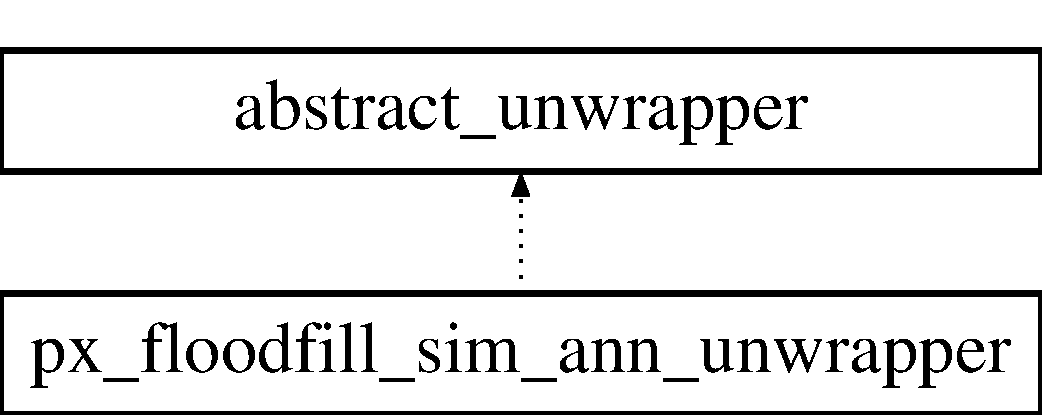
\includegraphics[height=2.000000cm]{classabstract__unwrapper}
\end{center}
\end{figure}
\subsection*{Public Member Functions}
\begin{DoxyCompactItemize}
\item 
virtual boost\-::shared\-\_\-ptr\\*
$<$ \hyperlink{classfloat__image}{float\-\_\-image} $>$ \hyperlink{classabstract__unwrapper_af7d5640f6f7e8beb7f7829c2260b94ee}{unwrap} (boost\-::shared\-\_\-ptr$<$ \hyperlink{classfloat__image}{float\-\_\-image} $>$ wrapped\-\_\-phase\-\_\-image)=0
\end{DoxyCompactItemize}


\subsection{Detailed Description}
This pure virtual class provides an interface for a general unwrapper that operates with boost smart pointers. 

\subsection{Member Function Documentation}
\hypertarget{classabstract__unwrapper_af7d5640f6f7e8beb7f7829c2260b94ee}{\index{abstract\-\_\-unwrapper@{abstract\-\_\-unwrapper}!unwrap@{unwrap}}
\index{unwrap@{unwrap}!abstract_unwrapper@{abstract\-\_\-unwrapper}}
\subsubsection[{unwrap}]{\setlength{\rightskip}{0pt plus 5cm}virtual boost\-::shared\-\_\-ptr$<${\bf float\-\_\-image}$>$ abstract\-\_\-unwrapper\-::unwrap (
\begin{DoxyParamCaption}
\item[{boost\-::shared\-\_\-ptr$<$ {\bf float\-\_\-image} $>$}]{wrapped\-\_\-phase\-\_\-image}
\end{DoxyParamCaption}
)\hspace{0.3cm}{\ttfamily [pure virtual]}}}\label{classabstract__unwrapper_af7d5640f6f7e8beb7f7829c2260b94ee}
An asbtract method for phase unwrapping. 
\begin{DoxyParams}{Parameters}
{\em wrapped\-\_\-phase\-\_\-image} & This image contains the wrapped phase data. \\
\hline
\end{DoxyParams}
\begin{DoxyReturn}{Returns}
A \hyperlink{classfloat__image}{float\-\_\-image} with the unwrapped phase data. The image will actually be a \hyperlink{classrow__major__float__image}{row\-\_\-major\-\_\-float\-\_\-image}. 
\end{DoxyReturn}


Implemented in \hyperlink{classpx__floodfill__sim__ann__unwrapper_a72c5c9cb7f151f50042b3d17f8b10b79}{px\-\_\-floodfill\-\_\-sim\-\_\-ann\-\_\-unwrapper}.



The documentation for this class was generated from the following file\-:\begin{DoxyCompactItemize}
\item 
include/algorithm/abstract\-\_\-unwrapper.\-h\end{DoxyCompactItemize}

\hypertarget{classcol__major__float__image}{\section{col\-\_\-major\-\_\-float\-\_\-image Class Reference}
\label{classcol__major__float__image}\index{col\-\_\-major\-\_\-float\-\_\-image@{col\-\_\-major\-\_\-float\-\_\-image}}
}
Inheritance diagram for col\-\_\-major\-\_\-float\-\_\-image\-:\begin{figure}[H]
\begin{center}
\leavevmode
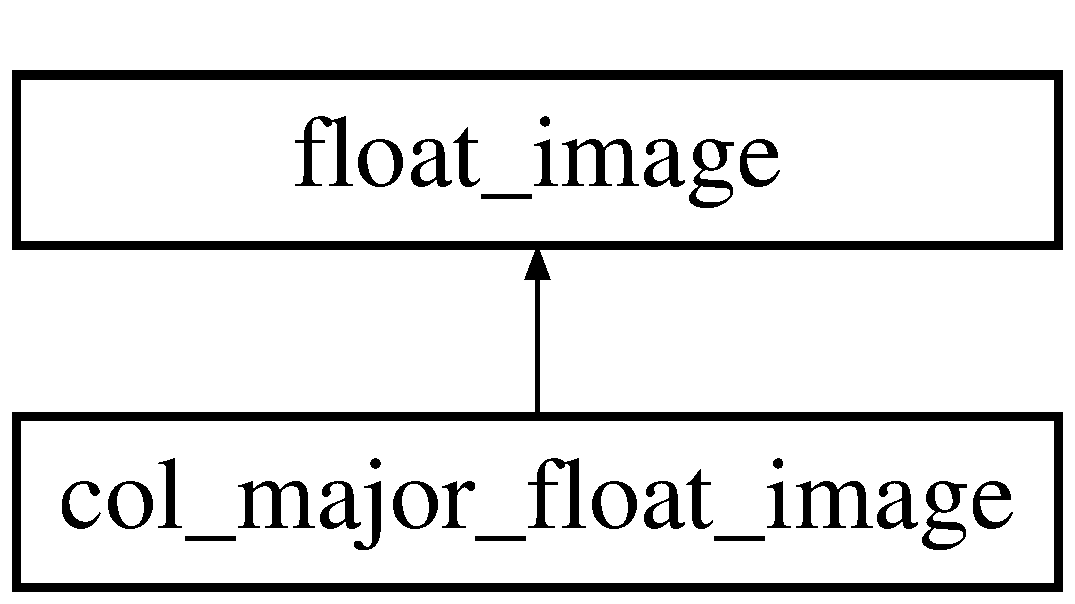
\includegraphics[height=2.000000cm]{classcol__major__float__image}
\end{center}
\end{figure}
\subsection*{Public Member Functions}
\begin{DoxyCompactItemize}
\item 
\hypertarget{classcol__major__float__image_afcf4d9a3059aca06c840338665077b53}{{\bfseries col\-\_\-major\-\_\-float\-\_\-image} (float $\ast$data, long width, long height)}\label{classcol__major__float__image_afcf4d9a3059aca06c840338665077b53}

\item 
\hyperlink{classcol__major__float__image_adeaacc7a78c0e3448597b34bff5b4c62}{col\-\_\-major\-\_\-float\-\_\-image} (long width, long height)
\item 
virtual float \& \hyperlink{classcol__major__float__image_a45315790d78a3d27559946f198129708}{operator()} (long w, long h)
\item 
\hypertarget{classcol__major__float__image_a83784cb35e0fef47a5f4b68fcf5a35c6}{virtual float {\bfseries operator()} (long w, long h) const }\label{classcol__major__float__image_a83784cb35e0fef47a5f4b68fcf5a35c6}

\end{DoxyCompactItemize}
\subsection*{Additional Inherited Members}


\subsection{Constructor \& Destructor Documentation}
\hypertarget{classcol__major__float__image_adeaacc7a78c0e3448597b34bff5b4c62}{\index{col\-\_\-major\-\_\-float\-\_\-image@{col\-\_\-major\-\_\-float\-\_\-image}!col\-\_\-major\-\_\-float\-\_\-image@{col\-\_\-major\-\_\-float\-\_\-image}}
\index{col\-\_\-major\-\_\-float\-\_\-image@{col\-\_\-major\-\_\-float\-\_\-image}!col_major_float_image@{col\-\_\-major\-\_\-float\-\_\-image}}
\subsubsection[{col\-\_\-major\-\_\-float\-\_\-image}]{\setlength{\rightskip}{0pt plus 5cm}col\-\_\-major\-\_\-float\-\_\-image\-::col\-\_\-major\-\_\-float\-\_\-image (
\begin{DoxyParamCaption}
\item[{long}]{width, }
\item[{long}]{height}
\end{DoxyParamCaption}
)\hspace{0.3cm}{\ttfamily [inline]}}}\label{classcol__major__float__image_adeaacc7a78c0e3448597b34bff5b4c62}
Generate image that reserves memory 
\begin{DoxyParams}{Parameters}
{\em width} & \\
\hline
{\em height} & \\
\hline
\end{DoxyParams}


\subsection{Member Function Documentation}
\hypertarget{classcol__major__float__image_a45315790d78a3d27559946f198129708}{\index{col\-\_\-major\-\_\-float\-\_\-image@{col\-\_\-major\-\_\-float\-\_\-image}!operator()@{operator()}}
\index{operator()@{operator()}!col_major_float_image@{col\-\_\-major\-\_\-float\-\_\-image}}
\subsubsection[{operator()}]{\setlength{\rightskip}{0pt plus 5cm}virtual float\& col\-\_\-major\-\_\-float\-\_\-image\-::operator() (
\begin{DoxyParamCaption}
\item[{long}]{w, }
\item[{long}]{h}
\end{DoxyParamCaption}
)\hspace{0.3cm}{\ttfamily [inline]}, {\ttfamily [virtual]}}}\label{classcol__major__float__image_a45315790d78a3d27559946f198129708}
Return element at position width = w, height = h, starting with (0,0) in upper left corner of the image. Implemented in child classes, see e.\-g. \hyperlink{classrow__major__float__image}{row\-\_\-major\-\_\-float\-\_\-image}. 

Implements \hyperlink{classfloat__image_a62e1446efb51fadcfeebf50568f9d1e9}{float\-\_\-image}.



The documentation for this class was generated from the following file\-:\begin{DoxyCompactItemize}
\item 
include/image/col\-\_\-major\-\_\-image.\-h\end{DoxyCompactItemize}

\input{class_ui_1_1digiholo_main_gui}
\input{classdigiholo_main_gui}
\hypertarget{struct_e_d_g_e}{\section{E\-D\-G\-E Struct Reference}
\label{struct_e_d_g_e}\index{E\-D\-G\-E@{E\-D\-G\-E}}
}
\subsection*{Public Attributes}
\begin{DoxyCompactItemize}
\item 
\hypertarget{struct_e_d_g_e_aeb147494099907a93ab92933235b5b2e}{float {\bfseries reliab}}\label{struct_e_d_g_e_aeb147494099907a93ab92933235b5b2e}

\item 
\hypertarget{struct_e_d_g_e_ab82d5a09f9a58543da71f2e8cbc821aa}{\hyperlink{struct_p_i_x_e_l}{P\-I\-X\-E\-L} $\ast$ {\bfseries pointer\-\_\-1}}\label{struct_e_d_g_e_ab82d5a09f9a58543da71f2e8cbc821aa}

\item 
\hypertarget{struct_e_d_g_e_a06ed3287e2c03f8b13d94b0845e065db}{\hyperlink{struct_p_i_x_e_l}{P\-I\-X\-E\-L} $\ast$ {\bfseries pointer\-\_\-2}}\label{struct_e_d_g_e_a06ed3287e2c03f8b13d94b0845e065db}

\item 
\hypertarget{struct_e_d_g_e_a29dca15549696bdc742e37df73de3482}{int {\bfseries increment}}\label{struct_e_d_g_e_a29dca15549696bdc742e37df73de3482}

\end{DoxyCompactItemize}


The documentation for this struct was generated from the following file\-:\begin{DoxyCompactItemize}
\item 
include/srncp/srncp\-\_\-unwrap.\-h\end{DoxyCompactItemize}

\hypertarget{classfloat__image}{\section{float\-\_\-image Class Reference}
\label{classfloat__image}\index{float\-\_\-image@{float\-\_\-image}}
}
Inheritance diagram for float\-\_\-image\-:\begin{figure}[H]
\begin{center}
\leavevmode
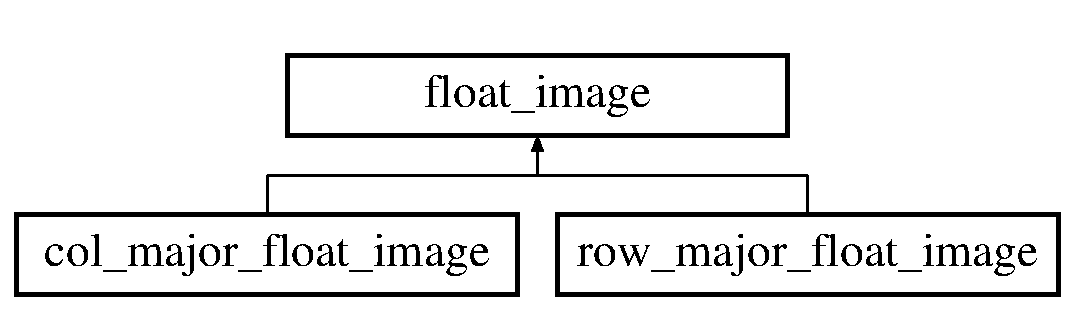
\includegraphics[height=2.000000cm]{classfloat__image}
\end{center}
\end{figure}
\subsection*{Public Member Functions}
\begin{DoxyCompactItemize}
\item 
\hyperlink{classfloat__image_a9e4ea7f98eb8c33e025cd21d61703c66}{float\-\_\-image} (long width, long height)
\item 
\hyperlink{classfloat__image_a4626247e8da835a5be04e346b577f85e}{float\-\_\-image} (float $\ast$data, long width, long height)
\item 
virtual long \hyperlink{classfloat__image_a08ba5e995f656dfebc5aaad0a9be390c}{get\-\_\-width} () const 
\item 
virtual long \hyperlink{classfloat__image_aeab41642909a0ee8d6e0ffcc2e7287b1}{get\-\_\-height} () const 
\item 
virtual float $\ast$ \hyperlink{classfloat__image_ab6dbf1f20614ba84f7b8f2c01b7aa3da}{get\-\_\-data\-\_\-pointer} ()
\item 
virtual float \& \hyperlink{classfloat__image_a62e1446efb51fadcfeebf50568f9d1e9}{operator()} (long w, long h)=0
\item 
\hypertarget{classfloat__image_ae3ae19180d1903bdeb0ffdb6f509a9f5}{virtual float {\bfseries operator()} (long w, long h) const =0}\label{classfloat__image_ae3ae19180d1903bdeb0ffdb6f509a9f5}

\item 
virtual void \hyperlink{classfloat__image_adffd8782a04ea4d764865aace1e43c93}{zero\-\_\-fill} ()
\item 
virtual bool \hyperlink{classfloat__image_a9cead12d50823ca313f6b7b16a57b092}{copy\-\_\-data\-\_\-to} (\hyperlink{classfloat__image}{float\-\_\-image} $\ast$img)
\item 
virtual void \hyperlink{classfloat__image_a3ef2df1d69f6791d2bef54636b625f82}{clear\-\_\-mem} ()
\item 
virtual float \hyperlink{classfloat__image_a53701b38abc94f8a707e8ceb2e6e71da}{get\-\_\-pixel} (long iw, long ih)
\item 
virtual void \hyperlink{classfloat__image_a97b520fc634fc4eb1930491b74d1f79b}{set\-\_\-pixel} (long iw, long ih, float val)
\end{DoxyCompactItemize}
\subsection*{Protected Attributes}
\begin{DoxyCompactItemize}
\item 
\hypertarget{classfloat__image_a43df6eebb483b16921cee23e80f61f5b}{float $\ast$ {\bfseries data}}\label{classfloat__image_a43df6eebb483b16921cee23e80f61f5b}

\item 
\hypertarget{classfloat__image_a92e539199f8cfa3c8ece64e2bdca54c7}{long {\bfseries width}}\label{classfloat__image_a92e539199f8cfa3c8ece64e2bdca54c7}

\item 
\hypertarget{classfloat__image_af7c859a1a77e6886adff0fd47976d069}{long {\bfseries height}}\label{classfloat__image_af7c859a1a77e6886adff0fd47976d069}

\end{DoxyCompactItemize}


\subsection{Detailed Description}
speichert ein 2\-D Bild, welches in einem 1\-D Datenvektor gespeichert wird. Die Ordnung des Datenvektors gibt die Klasse nicht vor. Es müssen auch nicht alle Daten hintereinander weg liegen. Die Zugriffsoperatoren sollen überladen werden, um eine bestimmte Art der Speicherung (z.\-b. row-\/major / column-\/major) oder sonstwas zu abstrahieren. Wichtig\-: Beim Aufruf des Destruktors des Bildes wird das entsprechende Array nicht freigegeben! 

\subsection{Constructor \& Destructor Documentation}
\hypertarget{classfloat__image_a9e4ea7f98eb8c33e025cd21d61703c66}{\index{float\-\_\-image@{float\-\_\-image}!float\-\_\-image@{float\-\_\-image}}
\index{float\-\_\-image@{float\-\_\-image}!float_image@{float\-\_\-image}}
\subsubsection[{float\-\_\-image}]{\setlength{\rightskip}{0pt plus 5cm}float\-\_\-image\-::float\-\_\-image (
\begin{DoxyParamCaption}
\item[{long}]{width, }
\item[{long}]{height}
\end{DoxyParamCaption}
)}}\label{classfloat__image_a9e4ea7f98eb8c33e025cd21d61703c66}
Create float image with and allocate data array! The data will not be zero filled. 
\begin{DoxyParams}{Parameters}
{\em width} & \\
\hline
{\em height} & \\
\hline
\end{DoxyParams}
\hypertarget{classfloat__image_a4626247e8da835a5be04e346b577f85e}{\index{float\-\_\-image@{float\-\_\-image}!float\-\_\-image@{float\-\_\-image}}
\index{float\-\_\-image@{float\-\_\-image}!float_image@{float\-\_\-image}}
\subsubsection[{float\-\_\-image}]{\setlength{\rightskip}{0pt plus 5cm}float\-\_\-image\-::float\-\_\-image (
\begin{DoxyParamCaption}
\item[{float $\ast$}]{data, }
\item[{long}]{width, }
\item[{long}]{height}
\end{DoxyParamCaption}
)}}\label{classfloat__image_a4626247e8da835a5be04e346b577f85e}
Create float image with specified data array. The image will operate on this array. 
\begin{DoxyParams}{Parameters}
{\em data} & \\
\hline
{\em width} & \\
\hline
{\em height} & \\
\hline
\end{DoxyParams}


\subsection{Member Function Documentation}
\hypertarget{classfloat__image_a3ef2df1d69f6791d2bef54636b625f82}{\index{float\-\_\-image@{float\-\_\-image}!clear\-\_\-mem@{clear\-\_\-mem}}
\index{clear\-\_\-mem@{clear\-\_\-mem}!float_image@{float\-\_\-image}}
\subsubsection[{clear\-\_\-mem}]{\setlength{\rightskip}{0pt plus 5cm}void float\-\_\-image\-::clear\-\_\-mem (
\begin{DoxyParamCaption}
{}
\end{DoxyParamCaption}
)\hspace{0.3cm}{\ttfamily [virtual]}}}\label{classfloat__image_a3ef2df1d69f6791d2bef54636b625f82}
Free memory associated with the image. This is not done when the destructor is called. \hypertarget{classfloat__image_a9cead12d50823ca313f6b7b16a57b092}{\index{float\-\_\-image@{float\-\_\-image}!copy\-\_\-data\-\_\-to@{copy\-\_\-data\-\_\-to}}
\index{copy\-\_\-data\-\_\-to@{copy\-\_\-data\-\_\-to}!float_image@{float\-\_\-image}}
\subsubsection[{copy\-\_\-data\-\_\-to}]{\setlength{\rightskip}{0pt plus 5cm}bool float\-\_\-image\-::copy\-\_\-data\-\_\-to (
\begin{DoxyParamCaption}
\item[{{\bf float\-\_\-image} $\ast$}]{img}
\end{DoxyParamCaption}
)\hspace{0.3cm}{\ttfamily [virtual]}}}\label{classfloat__image_a9cead12d50823ca313f6b7b16a57b092}
Copies the data from this image into the given image. Both images need to have the same dimensions. 
\begin{DoxyParams}{Parameters}
{\em img} & Data from this image is copied into img. \\
\hline
\end{DoxyParams}
\begin{DoxyReturn}{Returns}
true if successful, false if not. 
\end{DoxyReturn}
\hypertarget{classfloat__image_ab6dbf1f20614ba84f7b8f2c01b7aa3da}{\index{float\-\_\-image@{float\-\_\-image}!get\-\_\-data\-\_\-pointer@{get\-\_\-data\-\_\-pointer}}
\index{get\-\_\-data\-\_\-pointer@{get\-\_\-data\-\_\-pointer}!float_image@{float\-\_\-image}}
\subsubsection[{get\-\_\-data\-\_\-pointer}]{\setlength{\rightskip}{0pt plus 5cm}float $\ast$ float\-\_\-image\-::get\-\_\-data\-\_\-pointer (
\begin{DoxyParamCaption}
{}
\end{DoxyParamCaption}
)\hspace{0.3cm}{\ttfamily [virtual]}}}\label{classfloat__image_ab6dbf1f20614ba84f7b8f2c01b7aa3da}
\begin{DoxyReturn}{Returns}
pointer to data array 
\end{DoxyReturn}
\hypertarget{classfloat__image_aeab41642909a0ee8d6e0ffcc2e7287b1}{\index{float\-\_\-image@{float\-\_\-image}!get\-\_\-height@{get\-\_\-height}}
\index{get\-\_\-height@{get\-\_\-height}!float_image@{float\-\_\-image}}
\subsubsection[{get\-\_\-height}]{\setlength{\rightskip}{0pt plus 5cm}long float\-\_\-image\-::get\-\_\-height (
\begin{DoxyParamCaption}
{}
\end{DoxyParamCaption}
) const\hspace{0.3cm}{\ttfamily [virtual]}}}\label{classfloat__image_aeab41642909a0ee8d6e0ffcc2e7287b1}
\begin{DoxyReturn}{Returns}
image height 
\end{DoxyReturn}
\hypertarget{classfloat__image_a53701b38abc94f8a707e8ceb2e6e71da}{\index{float\-\_\-image@{float\-\_\-image}!get\-\_\-pixel@{get\-\_\-pixel}}
\index{get\-\_\-pixel@{get\-\_\-pixel}!float_image@{float\-\_\-image}}
\subsubsection[{get\-\_\-pixel}]{\setlength{\rightskip}{0pt plus 5cm}float float\-\_\-image\-::get\-\_\-pixel (
\begin{DoxyParamCaption}
\item[{long}]{iw, }
\item[{long}]{ih}
\end{DoxyParamCaption}
)\hspace{0.3cm}{\ttfamily [virtual]}}}\label{classfloat__image_a53701b38abc94f8a707e8ceb2e6e71da}
Get Pixel value at specified position. 
\begin{DoxyParams}{Parameters}
{\em iw} & \\
\hline
{\em ih} & \\
\hline
\end{DoxyParams}
\begin{DoxyReturn}{Returns}

\end{DoxyReturn}
\hypertarget{classfloat__image_a08ba5e995f656dfebc5aaad0a9be390c}{\index{float\-\_\-image@{float\-\_\-image}!get\-\_\-width@{get\-\_\-width}}
\index{get\-\_\-width@{get\-\_\-width}!float_image@{float\-\_\-image}}
\subsubsection[{get\-\_\-width}]{\setlength{\rightskip}{0pt plus 5cm}long float\-\_\-image\-::get\-\_\-width (
\begin{DoxyParamCaption}
{}
\end{DoxyParamCaption}
) const\hspace{0.3cm}{\ttfamily [virtual]}}}\label{classfloat__image_a08ba5e995f656dfebc5aaad0a9be390c}
\begin{DoxyReturn}{Returns}
image width 
\end{DoxyReturn}
\hypertarget{classfloat__image_a62e1446efb51fadcfeebf50568f9d1e9}{\index{float\-\_\-image@{float\-\_\-image}!operator()@{operator()}}
\index{operator()@{operator()}!float_image@{float\-\_\-image}}
\subsubsection[{operator()}]{\setlength{\rightskip}{0pt plus 5cm}virtual float\& float\-\_\-image\-::operator() (
\begin{DoxyParamCaption}
\item[{long}]{w, }
\item[{long}]{h}
\end{DoxyParamCaption}
)\hspace{0.3cm}{\ttfamily [pure virtual]}}}\label{classfloat__image_a62e1446efb51fadcfeebf50568f9d1e9}
Return element at position width = w, height = h, starting with (0,0) in upper left corner of the image. Implemented in child classes, see e.\-g. \hyperlink{classrow__major__float__image}{row\-\_\-major\-\_\-float\-\_\-image}. 

Implemented in \hyperlink{classcol__major__float__image_a45315790d78a3d27559946f198129708}{col\-\_\-major\-\_\-float\-\_\-image}, and \hyperlink{classrow__major__float__image_a04b9b253a3771e0963c839a9a85ccd99}{row\-\_\-major\-\_\-float\-\_\-image}.

\hypertarget{classfloat__image_a97b520fc634fc4eb1930491b74d1f79b}{\index{float\-\_\-image@{float\-\_\-image}!set\-\_\-pixel@{set\-\_\-pixel}}
\index{set\-\_\-pixel@{set\-\_\-pixel}!float_image@{float\-\_\-image}}
\subsubsection[{set\-\_\-pixel}]{\setlength{\rightskip}{0pt plus 5cm}void float\-\_\-image\-::set\-\_\-pixel (
\begin{DoxyParamCaption}
\item[{long}]{iw, }
\item[{long}]{ih, }
\item[{float}]{val}
\end{DoxyParamCaption}
)\hspace{0.3cm}{\ttfamily [virtual]}}}\label{classfloat__image_a97b520fc634fc4eb1930491b74d1f79b}
Set Pixel value at specified position. 
\begin{DoxyParams}{Parameters}
{\em iw} & \\
\hline
{\em ih} & \\
\hline
{\em val} & \\
\hline
\end{DoxyParams}
\begin{DoxyReturn}{Returns}

\end{DoxyReturn}
\hypertarget{classfloat__image_adffd8782a04ea4d764865aace1e43c93}{\index{float\-\_\-image@{float\-\_\-image}!zero\-\_\-fill@{zero\-\_\-fill}}
\index{zero\-\_\-fill@{zero\-\_\-fill}!float_image@{float\-\_\-image}}
\subsubsection[{zero\-\_\-fill}]{\setlength{\rightskip}{0pt plus 5cm}void float\-\_\-image\-::zero\-\_\-fill (
\begin{DoxyParamCaption}
{}
\end{DoxyParamCaption}
)\hspace{0.3cm}{\ttfamily [virtual]}}}\label{classfloat__image_adffd8782a04ea4d764865aace1e43c93}
Fill image with zeroes. 

The documentation for this class was generated from the following files\-:\begin{DoxyCompactItemize}
\item 
include/float\-\_\-image.\-h\item 
src/float\-\_\-image.\-cpp\end{DoxyCompactItemize}

\hypertarget{classgrad__fit__tile__unwrapper}{\section{grad\-\_\-fit\-\_\-tile\-\_\-unwrapper Class Reference}
\label{classgrad__fit__tile__unwrapper}\index{grad\-\_\-fit\-\_\-tile\-\_\-unwrapper@{grad\-\_\-fit\-\_\-tile\-\_\-unwrapper}}
}
Inheritance diagram for grad\-\_\-fit\-\_\-tile\-\_\-unwrapper\-:\begin{figure}[H]
\begin{center}
\leavevmode
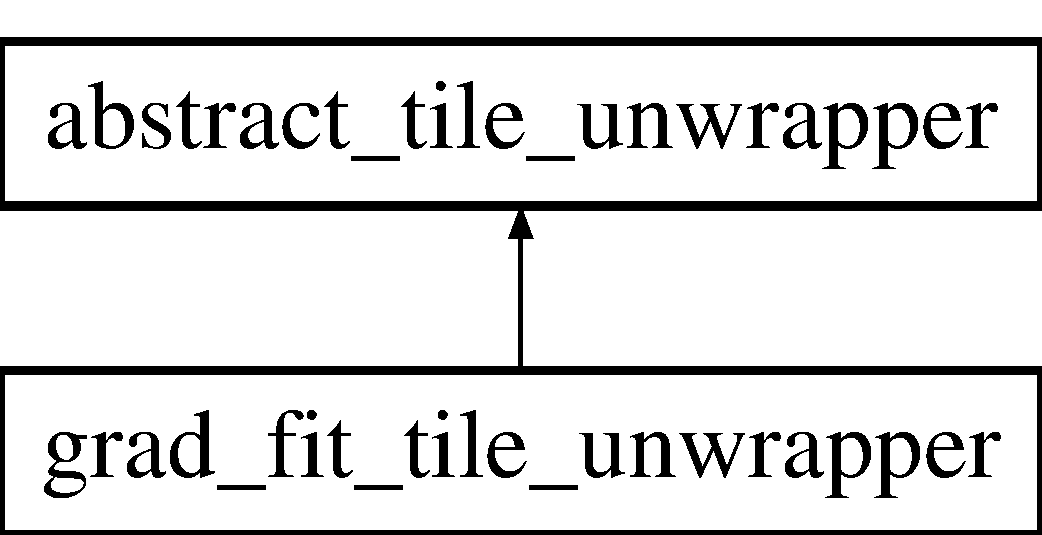
\includegraphics[height=2.000000cm]{classgrad__fit__tile__unwrapper}
\end{center}
\end{figure}
\subsection*{Public Member Functions}
\begin{DoxyCompactItemize}
\item 
\hypertarget{classgrad__fit__tile__unwrapper_a79033def7d478d1ef50b627b0663700d}{void {\bfseries unwrap} (sharedptr$<$ \hyperlink{classtile}{tile} $>$ t)}\label{classgrad__fit__tile__unwrapper_a79033def7d478d1ef50b627b0663700d}

\item 
virtual std\-::string \hyperlink{classgrad__fit__tile__unwrapper_a46a71a2adc53411289f792aae8c1b61c}{get\-\_\-name} ()
\item 
virtual void \hyperlink{classgrad__fit__tile__unwrapper_a62df2a6e799306b85f273a4f5aa43b4c}{usage\-\_\-help} ()
\end{DoxyCompactItemize}


\subsection{Member Function Documentation}
\hypertarget{classgrad__fit__tile__unwrapper_a46a71a2adc53411289f792aae8c1b61c}{\index{grad\-\_\-fit\-\_\-tile\-\_\-unwrapper@{grad\-\_\-fit\-\_\-tile\-\_\-unwrapper}!get\-\_\-name@{get\-\_\-name}}
\index{get\-\_\-name@{get\-\_\-name}!grad_fit_tile_unwrapper@{grad\-\_\-fit\-\_\-tile\-\_\-unwrapper}}
\subsubsection[{get\-\_\-name}]{\setlength{\rightskip}{0pt plus 5cm}std\-::string grad\-\_\-fit\-\_\-tile\-\_\-unwrapper\-::get\-\_\-name (
\begin{DoxyParamCaption}
{}
\end{DoxyParamCaption}
)\hspace{0.3cm}{\ttfamily [virtual]}}}\label{classgrad__fit__tile__unwrapper_a46a71a2adc53411289f792aae8c1b61c}
Return a name (with options) to set in the output file name 

Implements \hyperlink{classabstract__tile__unwrapper_ae70f69a703e622e5ab13eabcc91fca4d}{abstract\-\_\-tile\-\_\-unwrapper}.

\hypertarget{classgrad__fit__tile__unwrapper_a62df2a6e799306b85f273a4f5aa43b4c}{\index{grad\-\_\-fit\-\_\-tile\-\_\-unwrapper@{grad\-\_\-fit\-\_\-tile\-\_\-unwrapper}!usage\-\_\-help@{usage\-\_\-help}}
\index{usage\-\_\-help@{usage\-\_\-help}!grad_fit_tile_unwrapper@{grad\-\_\-fit\-\_\-tile\-\_\-unwrapper}}
\subsubsection[{usage\-\_\-help}]{\setlength{\rightskip}{0pt plus 5cm}void grad\-\_\-fit\-\_\-tile\-\_\-unwrapper\-::usage\-\_\-help (
\begin{DoxyParamCaption}
{}
\end{DoxyParamCaption}
)\hspace{0.3cm}{\ttfamily [virtual]}}}\label{classgrad__fit__tile__unwrapper_a62df2a6e799306b85f273a4f5aa43b4c}
Display a help on how to use this merger, in particular usage of merger-\/settings 

Implements \hyperlink{classabstract__tile__unwrapper_a469b36a7f302d5a2655631bbdb6f8daf}{abstract\-\_\-tile\-\_\-unwrapper}.



The documentation for this class was generated from the following files\-:\begin{DoxyCompactItemize}
\item 
include/algorithm/grad\-\_\-fit\-\_\-tile\-\_\-unwrapper.\-h\item 
src/algorithm/grad\-\_\-fit\-\_\-tile\-\_\-unwrapper.\-cpp\end{DoxyCompactItemize}

\hypertarget{classminimization__tile__unwrapper}{\section{minimization\-\_\-tile\-\_\-unwrapper Class Reference}
\label{classminimization__tile__unwrapper}\index{minimization\-\_\-tile\-\_\-unwrapper@{minimization\-\_\-tile\-\_\-unwrapper}}
}
Inheritance diagram for minimization\-\_\-tile\-\_\-unwrapper\-:\begin{figure}[H]
\begin{center}
\leavevmode
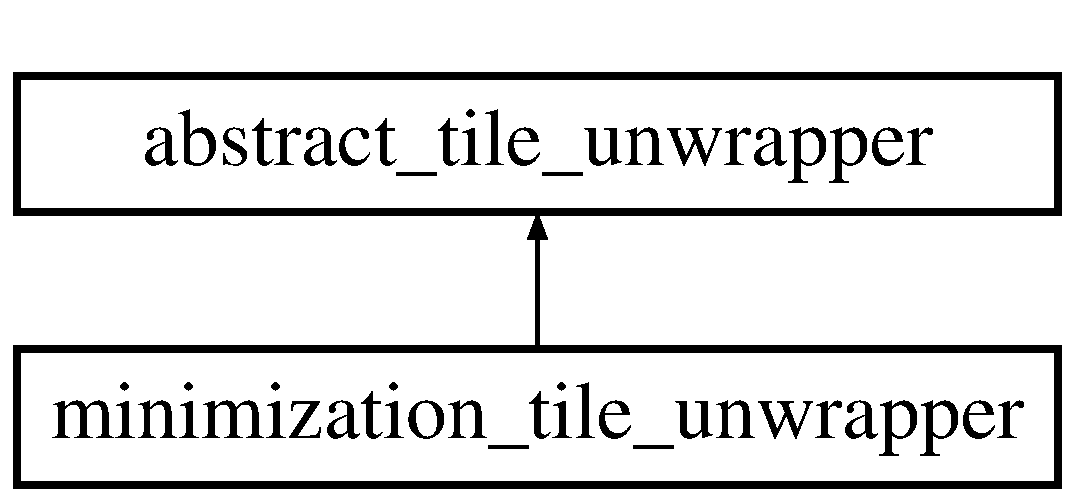
\includegraphics[height=2.000000cm]{classminimization__tile__unwrapper}
\end{center}
\end{figure}
\subsection*{Public Member Functions}
\begin{DoxyCompactItemize}
\item 
\hyperlink{classminimization__tile__unwrapper_acd1f71bbf4da842023eeb888ff07df07}{minimization\-\_\-tile\-\_\-unwrapper} (int max\-\_\-inter, float tol=0.\-0314)
\item 
virtual \hyperlink{classminimization__tile__unwrapper_a87733a219fdd57965ecccf833d6d8ea7}{$\sim$minimization\-\_\-tile\-\_\-unwrapper} ()
\item 
virtual void \hyperlink{classminimization__tile__unwrapper_a029e05336da3208ecb7a00ab553dd1c1}{unwrap} (\hyperlink{classtile}{tile} $\ast$t)
\end{DoxyCompactItemize}


\subsection{Detailed Description}
!! Diese Klasse soll mit G\-S\-L eine effizienteren Tile-\/\-Unwrap als der \hyperlink{class_strand__tile__unwrapper}{Strand\-\_\-tile\-\_\-unwrapper} durchführen. Es ist allerdings nicht so leicht, das Minimierungsproblem so zu verpacken, dass es mit Minimierungsroutinen gelöst werden kann. Man muss erstmal das Minimum eingrenzen... wie soll ich das möglichst effizient machen? 

\subsection{Constructor \& Destructor Documentation}
\hypertarget{classminimization__tile__unwrapper_acd1f71bbf4da842023eeb888ff07df07}{\index{minimization\-\_\-tile\-\_\-unwrapper@{minimization\-\_\-tile\-\_\-unwrapper}!minimization\-\_\-tile\-\_\-unwrapper@{minimization\-\_\-tile\-\_\-unwrapper}}
\index{minimization\-\_\-tile\-\_\-unwrapper@{minimization\-\_\-tile\-\_\-unwrapper}!minimization_tile_unwrapper@{minimization\-\_\-tile\-\_\-unwrapper}}
\subsubsection[{minimization\-\_\-tile\-\_\-unwrapper}]{\setlength{\rightskip}{0pt plus 5cm}minimization\-\_\-tile\-\_\-unwrapper\-::minimization\-\_\-tile\-\_\-unwrapper (
\begin{DoxyParamCaption}
\item[{int}]{max\-\_\-inter, }
\item[{float}]{tol = {\ttfamily 0.0314}}
\end{DoxyParamCaption}
)}}\label{classminimization__tile__unwrapper_acd1f71bbf4da842023eeb888ff07df07}
Constructor 
\begin{DoxyParams}{Parameters}
{\em max\-\_\-inter} & Max number of iterations for minimization \\
\hline
{\em tol} & Tolerance parameter as stopping criterion for minimization \\
\hline
\end{DoxyParams}
Allocate a Brent type minimizer; \hypertarget{classminimization__tile__unwrapper_a87733a219fdd57965ecccf833d6d8ea7}{\index{minimization\-\_\-tile\-\_\-unwrapper@{minimization\-\_\-tile\-\_\-unwrapper}!$\sim$minimization\-\_\-tile\-\_\-unwrapper@{$\sim$minimization\-\_\-tile\-\_\-unwrapper}}
\index{$\sim$minimization\-\_\-tile\-\_\-unwrapper@{$\sim$minimization\-\_\-tile\-\_\-unwrapper}!minimization_tile_unwrapper@{minimization\-\_\-tile\-\_\-unwrapper}}
\subsubsection[{$\sim$minimization\-\_\-tile\-\_\-unwrapper}]{\setlength{\rightskip}{0pt plus 5cm}minimization\-\_\-tile\-\_\-unwrapper\-::$\sim$minimization\-\_\-tile\-\_\-unwrapper (
\begin{DoxyParamCaption}
{}
\end{DoxyParamCaption}
)\hspace{0.3cm}{\ttfamily [virtual]}}}\label{classminimization__tile__unwrapper_a87733a219fdd57965ecccf833d6d8ea7}
Destruktor 

\subsection{Member Function Documentation}
\hypertarget{classminimization__tile__unwrapper_a029e05336da3208ecb7a00ab553dd1c1}{\index{minimization\-\_\-tile\-\_\-unwrapper@{minimization\-\_\-tile\-\_\-unwrapper}!unwrap@{unwrap}}
\index{unwrap@{unwrap}!minimization_tile_unwrapper@{minimization\-\_\-tile\-\_\-unwrapper}}
\subsubsection[{unwrap}]{\setlength{\rightskip}{0pt plus 5cm}void minimization\-\_\-tile\-\_\-unwrapper\-::unwrap (
\begin{DoxyParamCaption}
\item[{{\bf tile} $\ast$}]{t}
\end{DoxyParamCaption}
)\hspace{0.3cm}{\ttfamily [virtual]}}}\label{classminimization__tile__unwrapper_a029e05336da3208ecb7a00ab553dd1c1}
Diese Methode unwrappt eine einzelne tile. H\-I\-E\-R T\-W\-E\-A\-K MÖ\-G\-L\-I\-C\-H FÜ\-R R\-E\-L\-A\-T\-I\-V\-E\-S S\-T\-O\-P\-P\-I\-N\-G K\-R\-I\-T\-E\-R\-I\-U\-M. Ich habe es auf 0.\-0 gesetzt. Siehe auch G\-S\-L Reference Manual.

Implements \hyperlink{classabstract__tile__unwrapper_a8fdb3a4fdb7600f643f4af3c861ff296}{abstract\-\_\-tile\-\_\-unwrapper}.



The documentation for this class was generated from the following files\-:\begin{DoxyCompactItemize}
\item 
include/block\-\_\-srncp/minimization\-\_\-tile\-\_\-unwrapper.\-h\item 
src/block\-\_\-srncp/minimization\-\_\-tile\-\_\-unwrapper.\-cpp\end{DoxyCompactItemize}

\hypertarget{struct_p_i_x_e_l}{\section{P\-I\-X\-E\-L Struct Reference}
\label{struct_p_i_x_e_l}\index{P\-I\-X\-E\-L@{P\-I\-X\-E\-L}}
}
\subsection*{Public Attributes}
\begin{DoxyCompactItemize}
\item 
\hypertarget{struct_p_i_x_e_l_af8ced9ca3342f6d0fecbd4925bb4c62b}{int {\bfseries increment}}\label{struct_p_i_x_e_l_af8ced9ca3342f6d0fecbd4925bb4c62b}

\item 
\hypertarget{struct_p_i_x_e_l_a95ed27bafd239313e789998c59a7ca18}{int {\bfseries number\-\_\-of\-\_\-pixels\-\_\-in\-\_\-group}}\label{struct_p_i_x_e_l_a95ed27bafd239313e789998c59a7ca18}

\item 
\hypertarget{struct_p_i_x_e_l_afb696d11884328d3023274607b1c879d}{float {\bfseries value}}\label{struct_p_i_x_e_l_afb696d11884328d3023274607b1c879d}

\item 
\hypertarget{struct_p_i_x_e_l_a6d48d8353caf61a48d4219eadbb3f9db}{float {\bfseries reliability}}\label{struct_p_i_x_e_l_a6d48d8353caf61a48d4219eadbb3f9db}

\item 
\hypertarget{struct_p_i_x_e_l_a56925a4105feb07e5960df08a2a4b085}{int {\bfseries group}}\label{struct_p_i_x_e_l_a56925a4105feb07e5960df08a2a4b085}

\item 
\hypertarget{struct_p_i_x_e_l_a32322b80f38ec554722805c2544e5e63}{int {\bfseries new\-\_\-group}}\label{struct_p_i_x_e_l_a32322b80f38ec554722805c2544e5e63}

\item 
\hypertarget{struct_p_i_x_e_l_ace70c69fab3209527a85c5019d343b5f}{struct \hyperlink{struct_p_i_x_e_l}{P\-I\-X\-E\-L} $\ast$ {\bfseries head}}\label{struct_p_i_x_e_l_ace70c69fab3209527a85c5019d343b5f}

\item 
\hypertarget{struct_p_i_x_e_l_acc7295b17faa43230c5e4f2924c2981b}{struct \hyperlink{struct_p_i_x_e_l}{P\-I\-X\-E\-L} $\ast$ {\bfseries last}}\label{struct_p_i_x_e_l_acc7295b17faa43230c5e4f2924c2981b}

\item 
\hypertarget{struct_p_i_x_e_l_a30381a661bf0f90c628a647802987955}{struct \hyperlink{struct_p_i_x_e_l}{P\-I\-X\-E\-L} $\ast$ {\bfseries next}}\label{struct_p_i_x_e_l_a30381a661bf0f90c628a647802987955}

\end{DoxyCompactItemize}


The documentation for this struct was generated from the following file\-:\begin{DoxyCompactItemize}
\item 
include/srncp/srncp\-\_\-unwrap.\-h\end{DoxyCompactItemize}

\input{structqt__meta__stringdata__digiholo_main_gui__t}
\input{structqt__meta__stringdata___reconstruction_thread__t}
\input{class_reconstruction_thread}
\hypertarget{classrow__major__float__image}{\section{row\-\_\-major\-\_\-float\-\_\-image Class Reference}
\label{classrow__major__float__image}\index{row\-\_\-major\-\_\-float\-\_\-image@{row\-\_\-major\-\_\-float\-\_\-image}}
}
Inheritance diagram for row\-\_\-major\-\_\-float\-\_\-image\-:\begin{figure}[H]
\begin{center}
\leavevmode
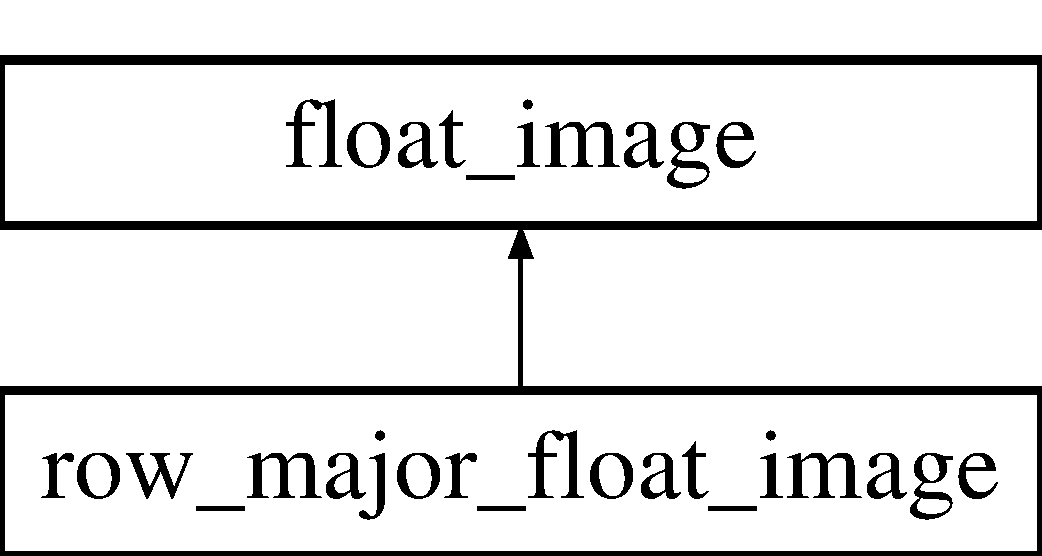
\includegraphics[height=2.000000cm]{classrow__major__float__image}
\end{center}
\end{figure}
\subsection*{Public Member Functions}
\begin{DoxyCompactItemize}
\item 
\hypertarget{classrow__major__float__image_a2aa84173f1aa9a37795e6b8d36642983}{{\bfseries row\-\_\-major\-\_\-float\-\_\-image} (float $\ast$data, long width, long height)}\label{classrow__major__float__image_a2aa84173f1aa9a37795e6b8d36642983}

\item 
\hyperlink{classrow__major__float__image_a918e2036b3d18fd6344f2edecd309891}{row\-\_\-major\-\_\-float\-\_\-image} (long width, long height)
\item 
virtual float \& \hyperlink{classrow__major__float__image_a04b9b253a3771e0963c839a9a85ccd99}{operator()} (long w, long h)
\item 
\hypertarget{classrow__major__float__image_af38e45798ef162384d75ad5c60cb40d0}{virtual float {\bfseries operator()} (long w, long h) const }\label{classrow__major__float__image_af38e45798ef162384d75ad5c60cb40d0}

\end{DoxyCompactItemize}
\subsection*{Additional Inherited Members}


\subsection{Constructor \& Destructor Documentation}
\hypertarget{classrow__major__float__image_a918e2036b3d18fd6344f2edecd309891}{\index{row\-\_\-major\-\_\-float\-\_\-image@{row\-\_\-major\-\_\-float\-\_\-image}!row\-\_\-major\-\_\-float\-\_\-image@{row\-\_\-major\-\_\-float\-\_\-image}}
\index{row\-\_\-major\-\_\-float\-\_\-image@{row\-\_\-major\-\_\-float\-\_\-image}!row_major_float_image@{row\-\_\-major\-\_\-float\-\_\-image}}
\subsubsection[{row\-\_\-major\-\_\-float\-\_\-image}]{\setlength{\rightskip}{0pt plus 5cm}row\-\_\-major\-\_\-float\-\_\-image\-::row\-\_\-major\-\_\-float\-\_\-image (
\begin{DoxyParamCaption}
\item[{long}]{width, }
\item[{long}]{height}
\end{DoxyParamCaption}
)\hspace{0.3cm}{\ttfamily [inline]}}}\label{classrow__major__float__image_a918e2036b3d18fd6344f2edecd309891}
Generate image that reserves memory 
\begin{DoxyParams}{Parameters}
{\em width} & \\
\hline
{\em height} & \\
\hline
\end{DoxyParams}


\subsection{Member Function Documentation}
\hypertarget{classrow__major__float__image_a04b9b253a3771e0963c839a9a85ccd99}{\index{row\-\_\-major\-\_\-float\-\_\-image@{row\-\_\-major\-\_\-float\-\_\-image}!operator()@{operator()}}
\index{operator()@{operator()}!row_major_float_image@{row\-\_\-major\-\_\-float\-\_\-image}}
\subsubsection[{operator()}]{\setlength{\rightskip}{0pt plus 5cm}float \& row\-\_\-major\-\_\-float\-\_\-image\-::operator() (
\begin{DoxyParamCaption}
\item[{long}]{w, }
\item[{long}]{h}
\end{DoxyParamCaption}
)\hspace{0.3cm}{\ttfamily [virtual]}}}\label{classrow__major__float__image_a04b9b253a3771e0963c839a9a85ccd99}
Return element at position width = w, height = h, starting with (0,0) in upper left corner of the image. Implemented in child classes, see e.\-g. \hyperlink{classrow__major__float__image}{row\-\_\-major\-\_\-float\-\_\-image}. 

Implements \hyperlink{classfloat__image_a62e1446efb51fadcfeebf50568f9d1e9}{float\-\_\-image}.



The documentation for this class was generated from the following files\-:\begin{DoxyCompactItemize}
\item 
include/row\-\_\-major\-\_\-float\-\_\-image.\-h\item 
src/row\-\_\-major\-\_\-float\-\_\-image.\-cpp\end{DoxyCompactItemize}

\hypertarget{classsimple1d__tile__merger}{\section{simple1d\-\_\-tile\-\_\-merger Class Reference}
\label{classsimple1d__tile__merger}\index{simple1d\-\_\-tile\-\_\-merger@{simple1d\-\_\-tile\-\_\-merger}}
}
Inheritance diagram for simple1d\-\_\-tile\-\_\-merger\-:\begin{figure}[H]
\begin{center}
\leavevmode
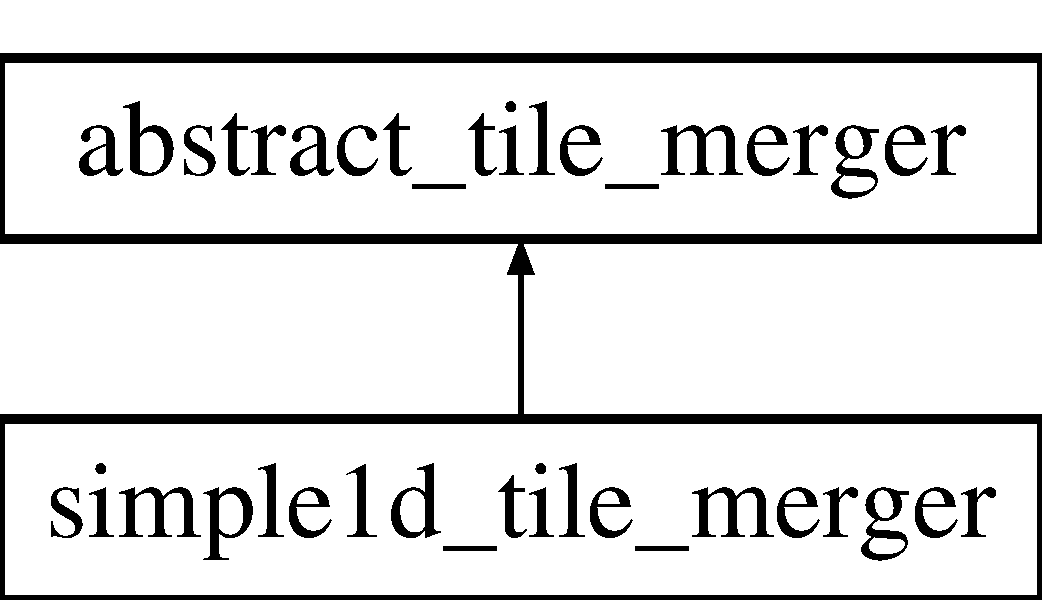
\includegraphics[height=2.000000cm]{classsimple1d__tile__merger}
\end{center}
\end{figure}
\subsection*{Public Member Functions}
\begin{DoxyCompactItemize}
\item 
\hyperlink{classsimple1d__tile__merger_a77f4873b02e49c780c80a80b204b094f}{simple1d\-\_\-tile\-\_\-merger} (float unwrap\-\_\-threshold)
\item 
virtual void \hyperlink{classsimple1d__tile__merger_a33c12f0c71ad8d05a4644d027060a17b}{merge\-\_\-tiles} (\hyperlink{classtesselated__image}{tesselated\-\_\-image} $\ast$t)
\end{DoxyCompactItemize}


\subsection{Constructor \& Destructor Documentation}
\hypertarget{classsimple1d__tile__merger_a77f4873b02e49c780c80a80b204b094f}{\index{simple1d\-\_\-tile\-\_\-merger@{simple1d\-\_\-tile\-\_\-merger}!simple1d\-\_\-tile\-\_\-merger@{simple1d\-\_\-tile\-\_\-merger}}
\index{simple1d\-\_\-tile\-\_\-merger@{simple1d\-\_\-tile\-\_\-merger}!simple1d_tile_merger@{simple1d\-\_\-tile\-\_\-merger}}
\subsubsection[{simple1d\-\_\-tile\-\_\-merger}]{\setlength{\rightskip}{0pt plus 5cm}simple1d\-\_\-tile\-\_\-merger\-::simple1d\-\_\-tile\-\_\-merger (
\begin{DoxyParamCaption}
\item[{float}]{unwrap\-\_\-threshold}
\end{DoxyParamCaption}
)}}\label{classsimple1d__tile__merger_a77f4873b02e49c780c80a80b204b094f}
Linear unwrapper based on 1d unwrapping of blocks. 
\begin{DoxyParams}{Parameters}
{\em unwrap\-\_\-threshold} & If this threshold is exceeded an unwrap between two blocks is performed. This parameter should be in \mbox{[}0,2\-P\-I\mbox{]}. \\
\hline
\end{DoxyParams}


\subsection{Member Function Documentation}
\hypertarget{classsimple1d__tile__merger_a33c12f0c71ad8d05a4644d027060a17b}{\index{simple1d\-\_\-tile\-\_\-merger@{simple1d\-\_\-tile\-\_\-merger}!merge\-\_\-tiles@{merge\-\_\-tiles}}
\index{merge\-\_\-tiles@{merge\-\_\-tiles}!simple1d_tile_merger@{simple1d\-\_\-tile\-\_\-merger}}
\subsubsection[{merge\-\_\-tiles}]{\setlength{\rightskip}{0pt plus 5cm}void simple1d\-\_\-tile\-\_\-merger\-::merge\-\_\-tiles (
\begin{DoxyParamCaption}
\item[{{\bf tesselated\-\_\-image} $\ast$}]{t}
\end{DoxyParamCaption}
)\hspace{0.3cm}{\ttfamily [virtual]}}}\label{classsimple1d__tile__merger_a33c12f0c71ad8d05a4644d027060a17b}
Merge tiles of tesselated image. The tiles have to be unwrapped inside themselves. This method unwraps the tiles with respect to each other. The phase discontinuity between each tile must be integer multiples of 2\-P\-I. 
\begin{DoxyParams}{Parameters}
{\em t} & \\
\hline
\end{DoxyParams}


Implements \hyperlink{classabstract__tile__merger_a60e28617e046734ef14ce15704a79680}{abstract\-\_\-tile\-\_\-merger}.



The documentation for this class was generated from the following files\-:\begin{DoxyCompactItemize}
\item 
include/block\-\_\-srncp/simple1d\-\_\-tile\-\_\-merger.\-h\item 
src/block\-\_\-srncp/simple1d\-\_\-tile\-\_\-merger.\-cpp\end{DoxyCompactItemize}

\input{classsmart__tile}
\input{classsmart__tile__junction}
\input{classsmart__tiled__image}
\input{classsmart__tilegroup}
\hypertarget{classsrncp__tile__merger}{\section{srncp\-\_\-tile\-\_\-merger Class Reference}
\label{classsrncp__tile__merger}\index{srncp\-\_\-tile\-\_\-merger@{srncp\-\_\-tile\-\_\-merger}}
}
Inheritance diagram for srncp\-\_\-tile\-\_\-merger\-:\begin{figure}[H]
\begin{center}
\leavevmode
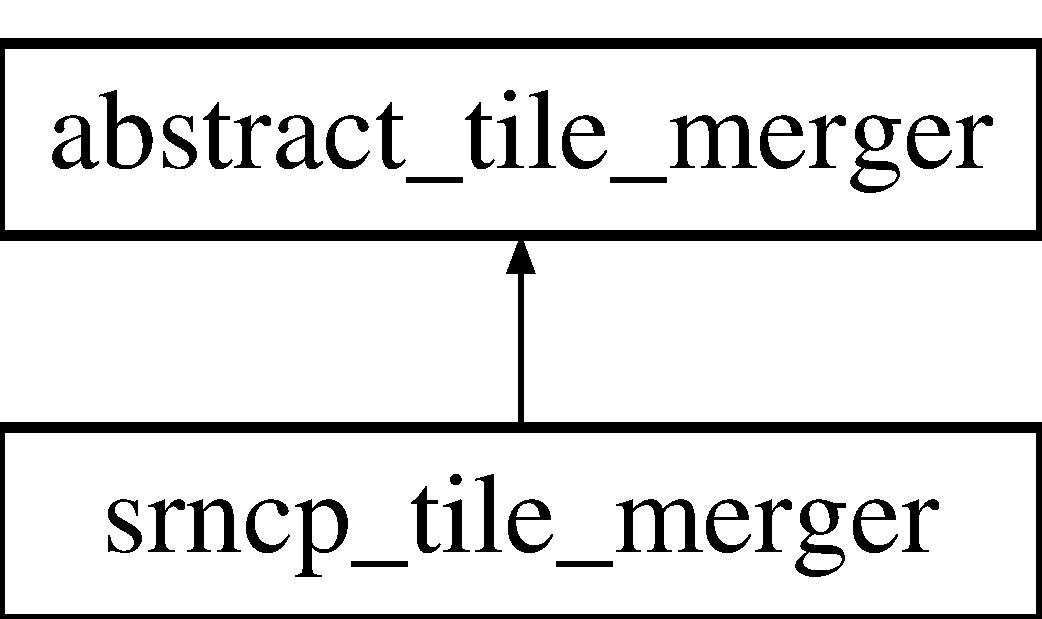
\includegraphics[height=2.000000cm]{classsrncp__tile__merger}
\end{center}
\end{figure}
\subsection*{Public Member Functions}
\begin{DoxyCompactItemize}
\item 
\hyperlink{classsrncp__tile__merger_aad58c1e54debf4ea2822cf07f6aa98c7}{srncp\-\_\-tile\-\_\-merger} (std\-::vector$<$ std\-::string $>$ msettings)
\item 
\hyperlink{classsrncp__tile__merger_a5b7ffbc05d851f3862a477cf17b31c53}{srncp\-\_\-tile\-\_\-merger} (boost\-::shared\-\_\-ptr$<$ \hyperlink{classabstract__reliability__calculator}{abstract\-\_\-reliability\-\_\-calculator} $>$ rc)
\item 
virtual void \hyperlink{classsrncp__tile__merger_ad8330c73633437c5f4860d837bf63345}{merge\-\_\-tiles} (boost\-::shared\-\_\-ptr$<$ \hyperlink{classtiled__image}{tiled\-\_\-image} $>$ ti)
\item 
virtual std\-::string \hyperlink{classsrncp__tile__merger_a7e6fb5b07129a1354a8d997161b210c4}{get\-\_\-name} ()
\item 
virtual void \hyperlink{classsrncp__tile__merger_ae57137ab8a1df19b86c28d3ff4aa1d9e}{usage\-\_\-help} ()
\end{DoxyCompactItemize}


\subsection{Constructor \& Destructor Documentation}
\hypertarget{classsrncp__tile__merger_aad58c1e54debf4ea2822cf07f6aa98c7}{\index{srncp\-\_\-tile\-\_\-merger@{srncp\-\_\-tile\-\_\-merger}!srncp\-\_\-tile\-\_\-merger@{srncp\-\_\-tile\-\_\-merger}}
\index{srncp\-\_\-tile\-\_\-merger@{srncp\-\_\-tile\-\_\-merger}!srncp_tile_merger@{srncp\-\_\-tile\-\_\-merger}}
\subsubsection[{srncp\-\_\-tile\-\_\-merger}]{\setlength{\rightskip}{0pt plus 5cm}srncp\-\_\-tile\-\_\-merger\-::srncp\-\_\-tile\-\_\-merger (
\begin{DoxyParamCaption}
\item[{std\-::vector$<$ std\-::string $>$}]{msettings}
\end{DoxyParamCaption}
)}}\label{classsrncp__tile__merger_aad58c1e54debf4ea2822cf07f6aa98c7}
Constructor used in the programm with settings as parameters 
\begin{DoxyParams}{Parameters}
{\em msettings} & settings for the merger \\
\hline
\end{DoxyParams}
\hypertarget{classsrncp__tile__merger_a5b7ffbc05d851f3862a477cf17b31c53}{\index{srncp\-\_\-tile\-\_\-merger@{srncp\-\_\-tile\-\_\-merger}!srncp\-\_\-tile\-\_\-merger@{srncp\-\_\-tile\-\_\-merger}}
\index{srncp\-\_\-tile\-\_\-merger@{srncp\-\_\-tile\-\_\-merger}!srncp_tile_merger@{srncp\-\_\-tile\-\_\-merger}}
\subsubsection[{srncp\-\_\-tile\-\_\-merger}]{\setlength{\rightskip}{0pt plus 5cm}srncp\-\_\-tile\-\_\-merger\-::srncp\-\_\-tile\-\_\-merger (
\begin{DoxyParamCaption}
\item[{boost\-::shared\-\_\-ptr$<$ {\bf abstract\-\_\-reliability\-\_\-calculator} $>$}]{rc}
\end{DoxyParamCaption}
)}}\label{classsrncp__tile__merger_a5b7ffbc05d851f3862a477cf17b31c53}
Explicit constructor with predefined reliability calculator 
\begin{DoxyParams}{Parameters}
{\em rc} & reliability calculator \\
\hline
\end{DoxyParams}


\subsection{Member Function Documentation}
\hypertarget{classsrncp__tile__merger_a7e6fb5b07129a1354a8d997161b210c4}{\index{srncp\-\_\-tile\-\_\-merger@{srncp\-\_\-tile\-\_\-merger}!get\-\_\-name@{get\-\_\-name}}
\index{get\-\_\-name@{get\-\_\-name}!srncp_tile_merger@{srncp\-\_\-tile\-\_\-merger}}
\subsubsection[{get\-\_\-name}]{\setlength{\rightskip}{0pt plus 5cm}std\-::string srncp\-\_\-tile\-\_\-merger\-::get\-\_\-name (
\begin{DoxyParamCaption}
{}
\end{DoxyParamCaption}
)\hspace{0.3cm}{\ttfamily [virtual]}}}\label{classsrncp__tile__merger_a7e6fb5b07129a1354a8d997161b210c4}
Return a name (with options) to set in the output file name 

Implements \hyperlink{classabstract__tile__merger_a12ec9d118912b3c571d61ff9649042c6}{abstract\-\_\-tile\-\_\-merger}.

\hypertarget{classsrncp__tile__merger_ad8330c73633437c5f4860d837bf63345}{\index{srncp\-\_\-tile\-\_\-merger@{srncp\-\_\-tile\-\_\-merger}!merge\-\_\-tiles@{merge\-\_\-tiles}}
\index{merge\-\_\-tiles@{merge\-\_\-tiles}!srncp_tile_merger@{srncp\-\_\-tile\-\_\-merger}}
\subsubsection[{merge\-\_\-tiles}]{\setlength{\rightskip}{0pt plus 5cm}void srncp\-\_\-tile\-\_\-merger\-::merge\-\_\-tiles (
\begin{DoxyParamCaption}
\item[{boost\-::shared\-\_\-ptr$<$ {\bf tiled\-\_\-image} $>$}]{ti}
\end{DoxyParamCaption}
)\hspace{0.3cm}{\ttfamily [virtual]}}}\label{classsrncp__tile__merger_ad8330c73633437c5f4860d837bf63345}
Merge all given tiles inside the tiled image 
\begin{DoxyParams}{Parameters}
{\em ti} & boost shared\-\_\-ptr to tiled image \\
\hline
\end{DoxyParams}


Implements \hyperlink{classabstract__tile__merger_a52ab494f77e495ab1a59b49e49c98db4}{abstract\-\_\-tile\-\_\-merger}.

\hypertarget{classsrncp__tile__merger_ae57137ab8a1df19b86c28d3ff4aa1d9e}{\index{srncp\-\_\-tile\-\_\-merger@{srncp\-\_\-tile\-\_\-merger}!usage\-\_\-help@{usage\-\_\-help}}
\index{usage\-\_\-help@{usage\-\_\-help}!srncp_tile_merger@{srncp\-\_\-tile\-\_\-merger}}
\subsubsection[{usage\-\_\-help}]{\setlength{\rightskip}{0pt plus 5cm}void srncp\-\_\-tile\-\_\-merger\-::usage\-\_\-help (
\begin{DoxyParamCaption}
{}
\end{DoxyParamCaption}
)\hspace{0.3cm}{\ttfamily [virtual]}}}\label{classsrncp__tile__merger_ae57137ab8a1df19b86c28d3ff4aa1d9e}
Display a help on how to use this merger, in particular usage of merger-\/settings 

Implements \hyperlink{classabstract__tile__merger_a7922b65624d12ef2d6c115218d2378b4}{abstract\-\_\-tile\-\_\-merger}.



The documentation for this class was generated from the following files\-:\begin{DoxyCompactItemize}
\item 
include/algorithm/srncp\-\_\-tile\-\_\-merger.\-h\item 
src/algorithm/srncp\-\_\-tile\-\_\-merger.\-cpp\end{DoxyCompactItemize}

\hypertarget{classsrncp__unwrapper}{\section{srncp\-\_\-unwrapper Class Reference}
\label{classsrncp__unwrapper}\index{srncp\-\_\-unwrapper@{srncp\-\_\-unwrapper}}
}
Inheritance diagram for srncp\-\_\-unwrapper\-:\begin{figure}[H]
\begin{center}
\leavevmode
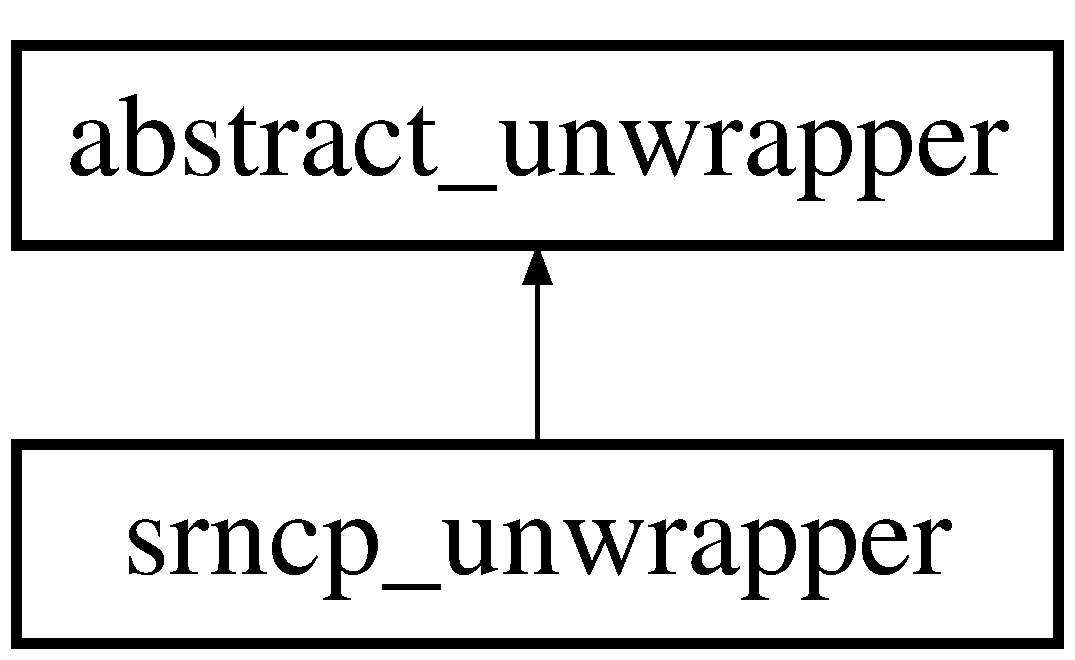
\includegraphics[height=2.000000cm]{classsrncp__unwrapper}
\end{center}
\end{figure}
\subsection*{Public Member Functions}
\begin{DoxyCompactItemize}
\item 
virtual bool \hyperlink{classsrncp__unwrapper_a9ca1b579f9ad3595daad40a7d9391376}{unwrap} (\hyperlink{classfloat__image}{float\-\_\-image} $\ast$wrapped, \hyperlink{classfloat__image}{float\-\_\-image} $\ast$unwrapped)
\end{DoxyCompactItemize}


\subsection{Detailed Description}
provides the functionality of the srncp unwrapper using the abstract unwrapper interface. \begin{DoxyAuthor}{Author}
g.\-antonopoulos 
\end{DoxyAuthor}


\subsection{Member Function Documentation}
\hypertarget{classsrncp__unwrapper_a9ca1b579f9ad3595daad40a7d9391376}{\index{srncp\-\_\-unwrapper@{srncp\-\_\-unwrapper}!unwrap@{unwrap}}
\index{unwrap@{unwrap}!srncp_unwrapper@{srncp\-\_\-unwrapper}}
\subsubsection[{unwrap}]{\setlength{\rightskip}{0pt plus 5cm}bool srncp\-\_\-unwrapper\-::unwrap (
\begin{DoxyParamCaption}
\item[{{\bf float\-\_\-image} $\ast$}]{wrapped\-\_\-phase\-\_\-image, }
\item[{{\bf float\-\_\-image} $\ast$}]{unwrapped\-\_\-phase\-\_\-image}
\end{DoxyParamCaption}
)\hspace{0.3cm}{\ttfamily [virtual]}}}\label{classsrncp__unwrapper_a9ca1b579f9ad3595daad40a7d9391376}
Abstrakte Methode für den Phase Unwrap 
\begin{DoxyParams}{Parameters}
{\em wrapped\-\_\-phase\-\_\-image} & Das Bild mit der Wrapped Phase Verteilung. \\
\hline
{\em unwrapped\-\_\-phase\-\_\-image} & Zeiger auf ein Bild mit Platz für die Unwrapped Phase Distribution. Muss gleiche größe wie wrapped phase haben!! \\
\hline
\end{DoxyParams}
\begin{DoxyReturn}{Returns}
true, wenn keine Fehler aufgetreten sind, sonst false. 
\end{DoxyReturn}


Implements \hyperlink{classabstract__unwrapper_a6d5c72cae9fcea45668cb02ddd3d9012}{abstract\-\_\-unwrapper}.



The documentation for this class was generated from the following files\-:\begin{DoxyCompactItemize}
\item 
include/srncp/srncp\-\_\-unwrap.\-h\item 
src/srncp/srncp\-\_\-unwrap.\-cpp\end{DoxyCompactItemize}

\hypertarget{class_strand__tile__unwrapper}{\section{Strand\-\_\-tile\-\_\-unwrapper Class Reference}
\label{class_strand__tile__unwrapper}\index{Strand\-\_\-tile\-\_\-unwrapper@{Strand\-\_\-tile\-\_\-unwrapper}}
}


{\ttfamily \#include $<$Strand\-\_\-tile\-\_\-unwrapper.\-h$>$}

Inheritance diagram for Strand\-\_\-tile\-\_\-unwrapper\-:\begin{figure}[H]
\begin{center}
\leavevmode
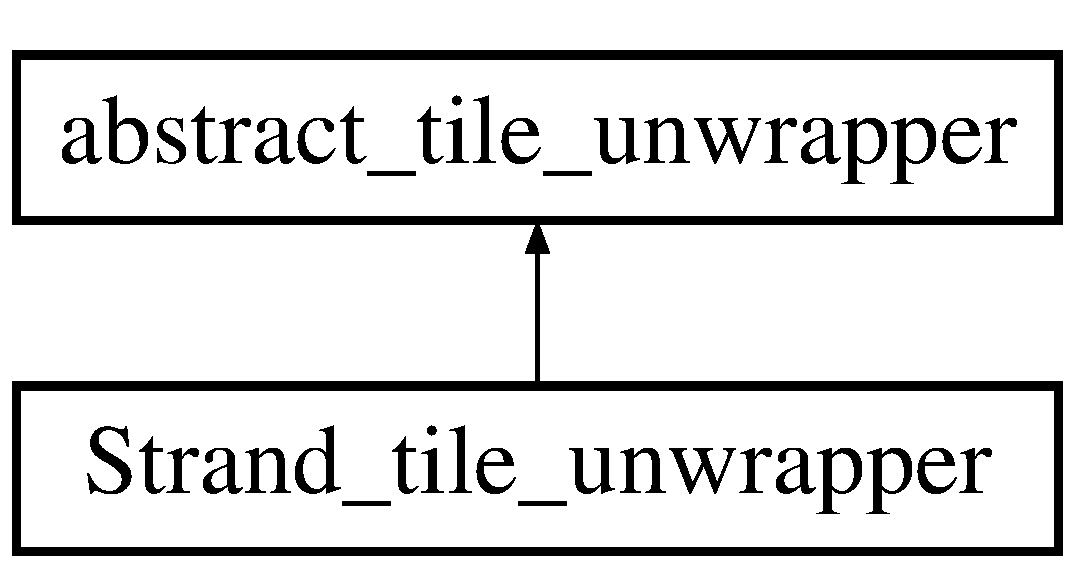
\includegraphics[height=2.000000cm]{class_strand__tile__unwrapper}
\end{center}
\end{figure}
\subsection*{Public Member Functions}
\begin{DoxyCompactItemize}
\item 
\hypertarget{class_strand__tile__unwrapper_afe8ff6109c61c4a150f4fdfd664459a4}{{\bfseries Strand\-\_\-tile\-\_\-unwrapper} (int N\-\_\-rho)}\label{class_strand__tile__unwrapper_afe8ff6109c61c4a150f4fdfd664459a4}

\item 
virtual void \hyperlink{class_strand__tile__unwrapper_a8a91a8867dc12db57db4f3960294f3ed}{unwrap} (\hyperlink{classtile}{tile} $\ast$t)
\end{DoxyCompactItemize}


\subsection{Detailed Description}
Unwrap single tile with the single block method from Strand et al.\-: \char`\"{}\-Two-\/\-Dimensional Phase Unwrapping Using a Block Least-\/\-Squares Method\char`\"{}, equations (4),(5) insbesondere 

\subsection{Member Function Documentation}
\hypertarget{class_strand__tile__unwrapper_a8a91a8867dc12db57db4f3960294f3ed}{\index{Strand\-\_\-tile\-\_\-unwrapper@{Strand\-\_\-tile\-\_\-unwrapper}!unwrap@{unwrap}}
\index{unwrap@{unwrap}!Strand_tile_unwrapper@{Strand\-\_\-tile\-\_\-unwrapper}}
\subsubsection[{unwrap}]{\setlength{\rightskip}{0pt plus 5cm}void Strand\-\_\-tile\-\_\-unwrapper\-::unwrap (
\begin{DoxyParamCaption}
\item[{{\bf tile} $\ast$}]{t}
\end{DoxyParamCaption}
)\hspace{0.3cm}{\ttfamily [virtual]}}}\label{class_strand__tile__unwrapper_a8a91a8867dc12db57db4f3960294f3ed}
!!!!!!!!!!!!!!!!!!!!!!!!!!!!!!!!!!!!!!!!!!!!! !!!!!!!!!!!!!!!!!!!!!!!!!!!!!!!!!!!!!!!!!!!!! !!!!!!!!!!!!!!!!!!!!!!!!!!!!!!!!!!!!!!!!!!!!! !!!!!!!!!!!!!!!!!!!!!!!!!!!!!!!!!!!!!!!!!!!!! 

Implements \hyperlink{classabstract__tile__unwrapper_a8fdb3a4fdb7600f643f4af3c861ff296}{abstract\-\_\-tile\-\_\-unwrapper}.



The documentation for this class was generated from the following files\-:\begin{DoxyCompactItemize}
\item 
include/block\-\_\-srncp/Strand\-\_\-tile\-\_\-unwrapper.\-h\item 
src/block\-\_\-srncp/Strand\-\_\-tile\-\_\-unwrapper.\-cpp\end{DoxyCompactItemize}

\hypertarget{class_takeda___f_f_t_w__fringe__analyser}{\section{Takeda\-\_\-\-F\-F\-T\-W\-\_\-fringe\-\_\-analyser Class Reference}
\label{class_takeda___f_f_t_w__fringe__analyser}\index{Takeda\-\_\-\-F\-F\-T\-W\-\_\-fringe\-\_\-analyser@{Takeda\-\_\-\-F\-F\-T\-W\-\_\-fringe\-\_\-analyser}}
}
Inheritance diagram for Takeda\-\_\-\-F\-F\-T\-W\-\_\-fringe\-\_\-analyser\-:\begin{figure}[H]
\begin{center}
\leavevmode
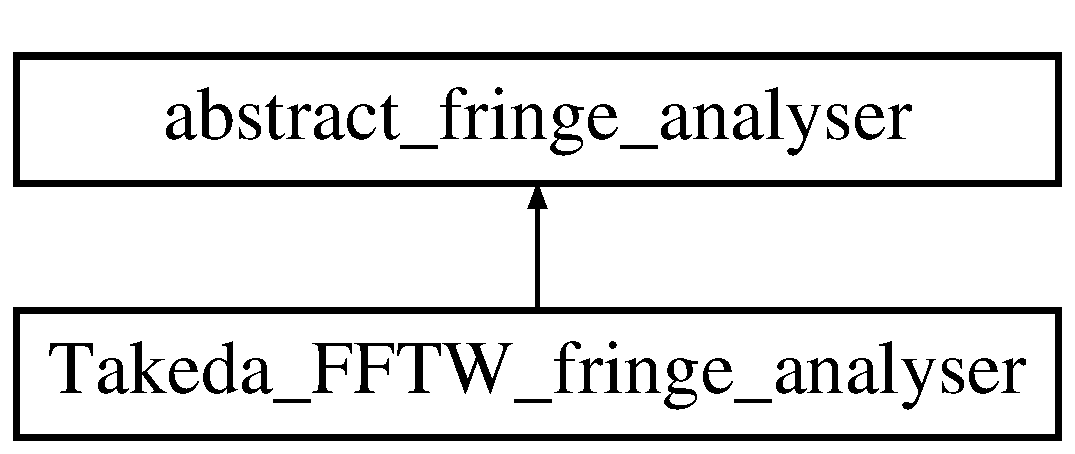
\includegraphics[height=2.000000cm]{class_takeda___f_f_t_w__fringe__analyser}
\end{center}
\end{figure}
\subsection*{Public Member Functions}
\begin{DoxyCompactItemize}
\item 
\hyperlink{class_takeda___f_f_t_w__fringe__analyser_a6512c3179a39f48bc25a7c9eb2abf1b0}{Takeda\-\_\-\-F\-F\-T\-W\-\_\-fringe\-\_\-analyser} (int width, int height, unsigned F\-L\-A\-G\-S=F\-F\-T\-W\-\_\-\-E\-S\-T\-I\-M\-A\-T\-E)
\item 
virtual bool \hyperlink{class_takeda___f_f_t_w__fringe__analyser_a0213cf26993557bf87b5c14d8b354582}{calc\-\_\-wrapped\-\_\-phase\-\_\-map} (\hyperlink{classfloat__image}{float\-\_\-image} $\ast$fringe\-\_\-img, \hyperlink{classfloat__image}{float\-\_\-image} $\ast$wrapped\-\_\-phase\-\_\-map)
\end{DoxyCompactItemize}
\subsection*{Static Public Attributes}
\begin{DoxyCompactItemize}
\item 
\hypertarget{class_takeda___f_f_t_w__fringe__analyser_a398b8368d2fd8a3803915d3142af6fc3}{static const float \hyperlink{class_takeda___f_f_t_w__fringe__analyser_a398b8368d2fd8a3803915d3142af6fc3}{C\-L\-I\-P\-P\-I\-N\-G\-\_\-\-F\-R\-A\-C\-T\-I\-O\-N} = 0.\-8f}\label{class_takeda___f_f_t_w__fringe__analyser_a398b8368d2fd8a3803915d3142af6fc3}

\begin{DoxyCompactList}\small\item\em Gibt an, wieviel Prozent des Abstand vonm der Nullfrequenz als clipping-\/radius verwendet werden. \end{DoxyCompactList}\end{DoxyCompactItemize}


\subsection{Detailed Description}
Wrapped Phase Map aus einem Interferenzbild mit einer beliebig orientierten Streifenmodulation nach Takeda et. al \char`\"{}\-Fourier-\/transform method of fringe-\/pattern analysis for computer-\/based topography and interferometry\char`\"{}. Dabei wird die F\-F\-T\-W verwendet, um die Fourier-\/\-Transformation durchzuführen. Die Bilder, welche übergeben werden, MÜ\-S\-S\-E\-N mit fftw\-\_\-malloc allociert worden sein. 

\subsection{Constructor \& Destructor Documentation}
\hypertarget{class_takeda___f_f_t_w__fringe__analyser_a6512c3179a39f48bc25a7c9eb2abf1b0}{\index{Takeda\-\_\-\-F\-F\-T\-W\-\_\-fringe\-\_\-analyser@{Takeda\-\_\-\-F\-F\-T\-W\-\_\-fringe\-\_\-analyser}!Takeda\-\_\-\-F\-F\-T\-W\-\_\-fringe\-\_\-analyser@{Takeda\-\_\-\-F\-F\-T\-W\-\_\-fringe\-\_\-analyser}}
\index{Takeda\-\_\-\-F\-F\-T\-W\-\_\-fringe\-\_\-analyser@{Takeda\-\_\-\-F\-F\-T\-W\-\_\-fringe\-\_\-analyser}!Takeda_FFTW_fringe_analyser@{Takeda\-\_\-\-F\-F\-T\-W\-\_\-fringe\-\_\-analyser}}
\subsubsection[{Takeda\-\_\-\-F\-F\-T\-W\-\_\-fringe\-\_\-analyser}]{\setlength{\rightskip}{0pt plus 5cm}Takeda\-\_\-\-F\-F\-T\-W\-\_\-fringe\-\_\-analyser\-::\-Takeda\-\_\-\-F\-F\-T\-W\-\_\-fringe\-\_\-analyser (
\begin{DoxyParamCaption}
\item[{int}]{width, }
\item[{int}]{height, }
\item[{unsigned}]{F\-L\-A\-G\-S = {\ttfamily FFTW\-\_\-ESTIMATE}}
\end{DoxyParamCaption}
)}}\label{class_takeda___f_f_t_w__fringe__analyser_a6512c3179a39f48bc25a7c9eb2abf1b0}
In dem Konstruktor wird ein Plan für ein Array mit width und height erstellt. Damit können dann alle weiteren Pläne schnell erstellt werden ausgeführt werden. Breite und Höhe der Bilder, die gerechnet werden sollen muss angegeben werden. Dies wird dazu benutzt, einmal einen Plan zu erstellen. Falls die Bilder in der calc\-\_\-wrapped\-\_\-phase\-\_\-map Methode nicht dieselbe Größe haben, wird eine exception geschmissen. 
\begin{DoxyParams}{Parameters}
{\em width} & Breite \\
\hline
{\em height} & Höhe \\
\hline
{\em flags} & \\
\hline
\end{DoxyParams}
Arrays für F\-F\-T\-W initialisieren 

\subsection{Member Function Documentation}
\hypertarget{class_takeda___f_f_t_w__fringe__analyser_a0213cf26993557bf87b5c14d8b354582}{\index{Takeda\-\_\-\-F\-F\-T\-W\-\_\-fringe\-\_\-analyser@{Takeda\-\_\-\-F\-F\-T\-W\-\_\-fringe\-\_\-analyser}!calc\-\_\-wrapped\-\_\-phase\-\_\-map@{calc\-\_\-wrapped\-\_\-phase\-\_\-map}}
\index{calc\-\_\-wrapped\-\_\-phase\-\_\-map@{calc\-\_\-wrapped\-\_\-phase\-\_\-map}!Takeda_FFTW_fringe_analyser@{Takeda\-\_\-\-F\-F\-T\-W\-\_\-fringe\-\_\-analyser}}
\subsubsection[{calc\-\_\-wrapped\-\_\-phase\-\_\-map}]{\setlength{\rightskip}{0pt plus 5cm}bool Takeda\-\_\-\-F\-F\-T\-W\-\_\-fringe\-\_\-analyser\-::calc\-\_\-wrapped\-\_\-phase\-\_\-map (
\begin{DoxyParamCaption}
\item[{{\bf float\-\_\-image} $\ast$}]{fringe\-\_\-img, }
\item[{{\bf float\-\_\-image} $\ast$}]{wrapped\-\_\-phase\-\_\-map}
\end{DoxyParamCaption}
)\hspace{0.3cm}{\ttfamily [virtual]}}}\label{class_takeda___f_f_t_w__fringe__analyser_a0213cf26993557bf87b5c14d8b354582}
Berechnung der Wrapped Phase Map aus einem Interferenzbild mit einer beliebig orientierten Streifenmodulation nach Takeda et. al \char`\"{}\-Fourier-\/transform method of fringe-\/pattern analysis for computer-\/based topography and interferometry\char`\"{}. 
\begin{DoxyParams}{Parameters}
{\em fringe\-\_\-pattern} & Das Interferenzbild. \\
\hline
{\em wrapped\-\_\-phase\-\_\-map} & Pointer mit Platz für die berechnete wrapped phase map. \\
\hline
\end{DoxyParams}
\begin{DoxyReturn}{Returns}
true, wenn keine Fehler aufgetreten sind, sonst false 
\end{DoxyReturn}


Implements \hyperlink{classabstract__fringe__analyser_a48f796b6b3d8dbf9dd66f5e5eaf98153}{abstract\-\_\-fringe\-\_\-analyser}.



The documentation for this class was generated from the following files\-:\begin{DoxyCompactItemize}
\item 
include/Takeda\-\_\-\-F\-F\-T\-W\-\_\-fringe\-\_\-analyser.\-h\item 
Takeda\-\_\-\-F\-F\-T\-W\-\_\-fringe\-\_\-analyser.\-cpp\end{DoxyCompactItemize}

\hypertarget{classtesselated__image}{\section{tesselated\-\_\-image Class Reference}
\label{classtesselated__image}\index{tesselated\-\_\-image@{tesselated\-\_\-image}}
}
\subsection*{Public Member Functions}
\begin{DoxyCompactItemize}
\item 
\hyperlink{classtesselated__image_a1046281f75fe41cd2395a26501c66c58}{tesselated\-\_\-image} ()
\item 
\hyperlink{classtesselated__image_a5ef32c85dbef869e3900a1d392c75662}{tesselated\-\_\-image} (\hyperlink{classfloat__image}{float\-\_\-image} $\ast$img, long tilecount\-\_\-width, long tilecount\-\_\-height)
\item 
\hyperlink{classtesselated__image}{tesselated\-\_\-image} \& \hyperlink{classtesselated__image_a253d97eb08831fdd271ba9c17d4da839}{operator=} (const \hyperlink{classtesselated__image}{tesselated\-\_\-image} \&t)
\item 
virtual \hyperlink{classtesselated__image_a0a5a7d1c9308ff5a381318e9be86944b}{$\sim$tesselated\-\_\-image} ()
\item 
\hypertarget{classtesselated__image_a61c89b7273500466cd229fc661262f3c}{\hyperlink{classtile}{tile} $\ast$ {\bfseries get\-\_\-tile\-\_\-ptr} (long w, long h)}\label{classtesselated__image_a61c89b7273500466cd229fc661262f3c}

\item 
long \hyperlink{classtesselated__image_a1a7dc52ce1d15494037c66fce2aea0a6}{get\-\_\-tile\-\_\-count\-\_\-width} () const 
\item 
long \hyperlink{classtesselated__image_ad7a9bc565d36ca41b7f373b3961ec8ce}{get\-\_\-tile\-\_\-count\-\_\-height} () const 
\item 
long \hyperlink{classtesselated__image_a091cf518fa74ff390f42e478253c6bf1}{get\-\_\-image\-\_\-width} () const 
\item 
long \hyperlink{classtesselated__image_a3316c95c95608fc1877225fac2db0c96}{get\-\_\-image\-\_\-height} () const 
\item 
void \hyperlink{classtesselated__image_a07e8990c014aea7fbb3e0ee7d3a7ebd2}{unwrap\-\_\-tiles} (\hyperlink{classabstract__tile__unwrapper}{abstract\-\_\-tile\-\_\-unwrapper} $\ast$u)
\end{DoxyCompactItemize}
\subsection*{Public Attributes}
\begin{DoxyCompactItemize}
\item 
\hypertarget{classtesselated__image_acc73733d08ac31133e707f1450e2933b}{\hyperlink{classtile}{tile} $\ast$$\ast$ {\bfseries image\-\_\-tiles}}\label{classtesselated__image_acc73733d08ac31133e707f1450e2933b}

\end{DoxyCompactItemize}


\subsection{Constructor \& Destructor Documentation}
\hypertarget{classtesselated__image_a1046281f75fe41cd2395a26501c66c58}{\index{tesselated\-\_\-image@{tesselated\-\_\-image}!tesselated\-\_\-image@{tesselated\-\_\-image}}
\index{tesselated\-\_\-image@{tesselated\-\_\-image}!tesselated_image@{tesselated\-\_\-image}}
\subsubsection[{tesselated\-\_\-image}]{\setlength{\rightskip}{0pt plus 5cm}tesselated\-\_\-image\-::tesselated\-\_\-image (
\begin{DoxyParamCaption}
{}
\end{DoxyParamCaption}
)}}\label{classtesselated__image_a1046281f75fe41cd2395a26501c66c58}
Standard constructor creates an empty tesselated images with all pointers set to N\-U\-L\-L and tilecount\-\_\-width and tilecount\-\_\-height of 0. \hypertarget{classtesselated__image_a5ef32c85dbef869e3900a1d392c75662}{\index{tesselated\-\_\-image@{tesselated\-\_\-image}!tesselated\-\_\-image@{tesselated\-\_\-image}}
\index{tesselated\-\_\-image@{tesselated\-\_\-image}!tesselated_image@{tesselated\-\_\-image}}
\subsubsection[{tesselated\-\_\-image}]{\setlength{\rightskip}{0pt plus 5cm}tesselated\-\_\-image\-::tesselated\-\_\-image (
\begin{DoxyParamCaption}
\item[{{\bf float\-\_\-image} $\ast$}]{img, }
\item[{long}]{tilecount\-\_\-width, }
\item[{long}]{tilecount\-\_\-height}
\end{DoxyParamCaption}
)}}\label{classtesselated__image_a5ef32c85dbef869e3900a1d392c75662}
Create a tiled image from an existing image. The tesselated image operates on the same memory as the original image. 
\begin{DoxyParams}{Parameters}
{\em img} & The image to be tesselated into tiles \\
\hline
{\em tilecount\-\_\-width} & Number if tiles in width direction. This number is not exactly adhered to, but the real number of tiles will be close. \\
\hline
{\em tilecount\-\_\-height} & Number of tiles in height direction. This number is not exactly adhered to, but the real number of tiles will be close. \\
\hline
\end{DoxyParams}
\hypertarget{classtesselated__image_a0a5a7d1c9308ff5a381318e9be86944b}{\index{tesselated\-\_\-image@{tesselated\-\_\-image}!$\sim$tesselated\-\_\-image@{$\sim$tesselated\-\_\-image}}
\index{$\sim$tesselated\-\_\-image@{$\sim$tesselated\-\_\-image}!tesselated_image@{tesselated\-\_\-image}}
\subsubsection[{$\sim$tesselated\-\_\-image}]{\setlength{\rightskip}{0pt plus 5cm}tesselated\-\_\-image\-::$\sim$tesselated\-\_\-image (
\begin{DoxyParamCaption}
{}
\end{DoxyParamCaption}
)\hspace{0.3cm}{\ttfamily [virtual]}}}\label{classtesselated__image_a0a5a7d1c9308ff5a381318e9be86944b}
Frees the memory associated with this image's tiles but does destroy the \hyperlink{classfloat__image}{float\-\_\-image} that this image operates on.

Free the memory opccupied by this object but not the underlying image. 

\subsection{Member Function Documentation}
\hypertarget{classtesselated__image_a3316c95c95608fc1877225fac2db0c96}{\index{tesselated\-\_\-image@{tesselated\-\_\-image}!get\-\_\-image\-\_\-height@{get\-\_\-image\-\_\-height}}
\index{get\-\_\-image\-\_\-height@{get\-\_\-image\-\_\-height}!tesselated_image@{tesselated\-\_\-image}}
\subsubsection[{get\-\_\-image\-\_\-height}]{\setlength{\rightskip}{0pt plus 5cm}long tesselated\-\_\-image\-::get\-\_\-image\-\_\-height (
\begin{DoxyParamCaption}
{}
\end{DoxyParamCaption}
) const}}\label{classtesselated__image_a3316c95c95608fc1877225fac2db0c96}
\begin{DoxyReturn}{Returns}
Image height in pixels 
\end{DoxyReturn}
\hypertarget{classtesselated__image_a091cf518fa74ff390f42e478253c6bf1}{\index{tesselated\-\_\-image@{tesselated\-\_\-image}!get\-\_\-image\-\_\-width@{get\-\_\-image\-\_\-width}}
\index{get\-\_\-image\-\_\-width@{get\-\_\-image\-\_\-width}!tesselated_image@{tesselated\-\_\-image}}
\subsubsection[{get\-\_\-image\-\_\-width}]{\setlength{\rightskip}{0pt plus 5cm}long tesselated\-\_\-image\-::get\-\_\-image\-\_\-width (
\begin{DoxyParamCaption}
{}
\end{DoxyParamCaption}
) const}}\label{classtesselated__image_a091cf518fa74ff390f42e478253c6bf1}
\begin{DoxyReturn}{Returns}
Image width in pixels 
\end{DoxyReturn}
\hypertarget{classtesselated__image_ad7a9bc565d36ca41b7f373b3961ec8ce}{\index{tesselated\-\_\-image@{tesselated\-\_\-image}!get\-\_\-tile\-\_\-count\-\_\-height@{get\-\_\-tile\-\_\-count\-\_\-height}}
\index{get\-\_\-tile\-\_\-count\-\_\-height@{get\-\_\-tile\-\_\-count\-\_\-height}!tesselated_image@{tesselated\-\_\-image}}
\subsubsection[{get\-\_\-tile\-\_\-count\-\_\-height}]{\setlength{\rightskip}{0pt plus 5cm}long tesselated\-\_\-image\-::get\-\_\-tile\-\_\-count\-\_\-height (
\begin{DoxyParamCaption}
{}
\end{DoxyParamCaption}
) const}}\label{classtesselated__image_ad7a9bc565d36ca41b7f373b3961ec8ce}
\begin{DoxyReturn}{Returns}
Number of tiles in height direction. 
\end{DoxyReturn}
\hypertarget{classtesselated__image_a1a7dc52ce1d15494037c66fce2aea0a6}{\index{tesselated\-\_\-image@{tesselated\-\_\-image}!get\-\_\-tile\-\_\-count\-\_\-width@{get\-\_\-tile\-\_\-count\-\_\-width}}
\index{get\-\_\-tile\-\_\-count\-\_\-width@{get\-\_\-tile\-\_\-count\-\_\-width}!tesselated_image@{tesselated\-\_\-image}}
\subsubsection[{get\-\_\-tile\-\_\-count\-\_\-width}]{\setlength{\rightskip}{0pt plus 5cm}long tesselated\-\_\-image\-::get\-\_\-tile\-\_\-count\-\_\-width (
\begin{DoxyParamCaption}
{}
\end{DoxyParamCaption}
) const}}\label{classtesselated__image_a1a7dc52ce1d15494037c66fce2aea0a6}
\begin{DoxyReturn}{Returns}
Number of tiles in width-\/direction. 
\end{DoxyReturn}
\hypertarget{classtesselated__image_a253d97eb08831fdd271ba9c17d4da839}{\index{tesselated\-\_\-image@{tesselated\-\_\-image}!operator=@{operator=}}
\index{operator=@{operator=}!tesselated_image@{tesselated\-\_\-image}}
\subsubsection[{operator=}]{\setlength{\rightskip}{0pt plus 5cm}{\bf tesselated\-\_\-image} \& tesselated\-\_\-image\-::operator= (
\begin{DoxyParamCaption}
\item[{const {\bf tesselated\-\_\-image} \&}]{t}
\end{DoxyParamCaption}
)}}\label{classtesselated__image_a253d97eb08831fdd271ba9c17d4da839}
Makes the L-\/value point to the same \hyperlink{classfloat__image}{float\-\_\-image} as the R-\/value but generates a new set of tiles for this image that are independent of the R-\/value's tiles. 
\begin{DoxyParams}{Parameters}
{\em t} & \\
\hline
\end{DoxyParams}
\begin{DoxyReturn}{Returns}

\end{DoxyReturn}
\hypertarget{classtesselated__image_a07e8990c014aea7fbb3e0ee7d3a7ebd2}{\index{tesselated\-\_\-image@{tesselated\-\_\-image}!unwrap\-\_\-tiles@{unwrap\-\_\-tiles}}
\index{unwrap\-\_\-tiles@{unwrap\-\_\-tiles}!tesselated_image@{tesselated\-\_\-image}}
\subsubsection[{unwrap\-\_\-tiles}]{\setlength{\rightskip}{0pt plus 5cm}void tesselated\-\_\-image\-::unwrap\-\_\-tiles (
\begin{DoxyParamCaption}
\item[{{\bf abstract\-\_\-tile\-\_\-unwrapper} $\ast$}]{u}
\end{DoxyParamCaption}
)}}\label{classtesselated__image_a07e8990c014aea7fbb3e0ee7d3a7ebd2}
Unwraps all tiles using the unwrap method given by the instance of the \hyperlink{classabstract__tile__unwrapper}{abstract\-\_\-tile\-\_\-unwrapper} 

The documentation for this class was generated from the following files\-:\begin{DoxyCompactItemize}
\item 
include/block\-\_\-srncp/tesselated\-\_\-image.\-h\item 
src/block\-\_\-srncp/tesselated\-\_\-image.\-cpp\end{DoxyCompactItemize}

\hypertarget{classtile}{\section{tile Class Reference}
\label{classtile}\index{tile@{tile}}
}
\subsection*{Public Member Functions}
\begin{DoxyCompactItemize}
\item 
void \hyperlink{classtile_aba3ebab4ffdbfdb86d9077b6c1510ac3}{clear\-\_\-mem} ()
\item 
\hyperlink{classtile_a4a11ab1e126b8f5a39145836fa15960d}{tile} (long max\-\_\-width, long max\-\_\-height)
\item 
\hyperlink{classtile_afbef14bff799cec1be0b2d504d66507b}{$\sim$tile} ()
\item 
\hypertarget{classtile_aa0eeadf75c401536efe4c07a8ddee4ab}{float \& \hyperlink{classtile_aa0eeadf75c401536efe4c07a8ddee4ab}{operator()} (long w, long h)}\label{classtile_aa0eeadf75c401536efe4c07a8ddee4ab}

\begin{DoxyCompactList}\small\item\em Access element of this tile at (w,h) \end{DoxyCompactList}\item 
\hypertarget{classtile_a9ff4c62c4eafa1e5ad077e60bc9abd0c}{float \hyperlink{classtile_a9ff4c62c4eafa1e5ad077e60bc9abd0c}{operator()} (long w, long h) const }\label{classtile_a9ff4c62c4eafa1e5ad077e60bc9abd0c}

\begin{DoxyCompactList}\small\item\em Access value of the element of this tile at (w,h) \end{DoxyCompactList}\item 
\hyperlink{classtile}{tile} \& \hyperlink{classtile_a044a719e0369d7b03ee81bdaf917ce96}{add\-\_\-value} (float value)
\item 
\hyperlink{classtile}{tile} \& \hyperlink{classtile_aa061c1fdcce1723f641355e9a884d329}{multiply} (float value)
\item 
\hyperlink{classtile}{tile} \& \hyperlink{classtile_a0e331de98d713a293c2d09524ceb2abb}{wrap} ()
\begin{DoxyCompactList}\small\item\em Only works if pixelvalue is in \mbox{[}-\/\-P\-I,P\-I\mbox{]} and val is in \mbox{[}-\/2\-P\-I,2\-P\-I\mbox{]}. \end{DoxyCompactList}\item 
\hyperlink{classtile}{tile} \& \hyperlink{classtile_a04907d189cf875a5749d751a8af1c7a9}{rewrap} (float val)
\item 
float $\ast$ \hyperlink{classtile_ab3b683d2fea9c14a8fb5fc6fb02cc14d}{copy\-\_\-data} () const 
\item 
long \hyperlink{classtile_ab17cd2ca85fb73ee40612f543dea083c}{get\-\_\-width} () const 
\item 
long \hyperlink{classtile_aa7077bc22ada6ea7e524d9d8e44431a1}{get\-\_\-height} () const 
\item 
void \hyperlink{classtile_a5f50600c8e541aa5ae85340d67fa9313}{generate\-\_\-from\-\_\-image} (\hyperlink{classfloat__image}{float\-\_\-image} $\ast$img, long tile\-\_\-max\-\_\-width, long tile\-\_\-max\-\_\-height, long iw, long ih)
\item 
float \hyperlink{classtile_a7a510ae32ed8f009d45adcc3714f2639}{calc\-\_\-mean} () const 
\item 
bool \hyperlink{classtile_a2c793b844fbbf58ab99fa1be5bdce744}{has\-\_\-group} ()
\item 
\hyperlink{classtilegroup}{tilegroup} $\ast$ \hyperlink{classtile_a11a5f9f4ccd3999489d284e1af38c192}{get\-\_\-tilegroup} ()
\end{DoxyCompactItemize}
\subsection*{Friends}
\begin{DoxyCompactItemize}
\item 
\hypertarget{classtile_a2fa7ac0b19bb84e1e68b73be2631ac2f}{class {\bfseries tilegroup}}\label{classtile_a2fa7ac0b19bb84e1e68b73be2631ac2f}

\end{DoxyCompactItemize}


\subsection{Detailed Description}
Unterteilung eines Bildes in Kacheln (tiles). Die Daten der Tiles sind nicht hintereinander im Speicher abgelegt, darum kann sie auch nicht von \hyperlink{classfloat__image}{float\-\_\-image} abgeleitet sein. 

\subsection{Constructor \& Destructor Documentation}
\hypertarget{classtile_a4a11ab1e126b8f5a39145836fa15960d}{\index{tile@{tile}!tile@{tile}}
\index{tile@{tile}!tile@{tile}}
\subsubsection[{tile}]{\setlength{\rightskip}{0pt plus 5cm}tile\-::tile (
\begin{DoxyParamCaption}
\item[{long}]{max\-\_\-width, }
\item[{long}]{max\-\_\-height}
\end{DoxyParamCaption}
)}}\label{classtile_a4a11ab1e126b8f5a39145836fa15960d}
Create a tile that reserves memory for pointers to (max\-\_\-width)X(max\-\_\-height) elements \hypertarget{classtile_afbef14bff799cec1be0b2d504d66507b}{\index{tile@{tile}!$\sim$tile@{$\sim$tile}}
\index{$\sim$tile@{$\sim$tile}!tile@{tile}}
\subsubsection[{$\sim$tile}]{\setlength{\rightskip}{0pt plus 5cm}tile\-::$\sim$tile (
\begin{DoxyParamCaption}
{}
\end{DoxyParamCaption}
)}}\label{classtile_afbef14bff799cec1be0b2d504d66507b}
Does not do anything. Call free to free mem. 

\subsection{Member Function Documentation}
\hypertarget{classtile_a044a719e0369d7b03ee81bdaf917ce96}{\index{tile@{tile}!add\-\_\-value@{add\-\_\-value}}
\index{add\-\_\-value@{add\-\_\-value}!tile@{tile}}
\subsubsection[{add\-\_\-value}]{\setlength{\rightskip}{0pt plus 5cm}{\bf tile} \& tile\-::add\-\_\-value (
\begin{DoxyParamCaption}
\item[{float}]{value}
\end{DoxyParamCaption}
)}}\label{classtile_a044a719e0369d7b03ee81bdaf917ce96}
Add a specified number to all pixels in the tile. 
\begin{DoxyParams}{Parameters}
{\em value} & The value to add. \\
\hline
\end{DoxyParams}
\hypertarget{classtile_a7a510ae32ed8f009d45adcc3714f2639}{\index{tile@{tile}!calc\-\_\-mean@{calc\-\_\-mean}}
\index{calc\-\_\-mean@{calc\-\_\-mean}!tile@{tile}}
\subsubsection[{calc\-\_\-mean}]{\setlength{\rightskip}{0pt plus 5cm}float tile\-::calc\-\_\-mean (
\begin{DoxyParamCaption}
{}
\end{DoxyParamCaption}
) const}}\label{classtile_a7a510ae32ed8f009d45adcc3714f2639}
Calculate mean value of pixel values in tile. \begin{DoxyReturn}{Returns}
mean. 
\end{DoxyReturn}
\hypertarget{classtile_aba3ebab4ffdbfdb86d9077b6c1510ac3}{\index{tile@{tile}!clear\-\_\-mem@{clear\-\_\-mem}}
\index{clear\-\_\-mem@{clear\-\_\-mem}!tile@{tile}}
\subsubsection[{clear\-\_\-mem}]{\setlength{\rightskip}{0pt plus 5cm}void tile\-::clear\-\_\-mem (
\begin{DoxyParamCaption}
{}
\end{DoxyParamCaption}
)}}\label{classtile_aba3ebab4ffdbfdb86d9077b6c1510ac3}
Hier wird nur der blockierte Speicher und nicht die Bildinformation auf die gezeigt wird gelöscht. \hypertarget{classtile_ab3b683d2fea9c14a8fb5fc6fb02cc14d}{\index{tile@{tile}!copy\-\_\-data@{copy\-\_\-data}}
\index{copy\-\_\-data@{copy\-\_\-data}!tile@{tile}}
\subsubsection[{copy\-\_\-data}]{\setlength{\rightskip}{0pt plus 5cm}float $\ast$ tile\-::copy\-\_\-data (
\begin{DoxyParamCaption}
{}
\end{DoxyParamCaption}
) const}}\label{classtile_ab3b683d2fea9c14a8fb5fc6fb02cc14d}
This methods allcocates memory for a 1\-D Array and copies the data that this tile points to into this array in a row (width) major fashion. The pointer to the copy of the data has to be deleted to avoid memory leaks. This is a nice little helper method. \begin{DoxyReturn}{Returns}

\end{DoxyReturn}
\hypertarget{classtile_a5f50600c8e541aa5ae85340d67fa9313}{\index{tile@{tile}!generate\-\_\-from\-\_\-image@{generate\-\_\-from\-\_\-image}}
\index{generate\-\_\-from\-\_\-image@{generate\-\_\-from\-\_\-image}!tile@{tile}}
\subsubsection[{generate\-\_\-from\-\_\-image}]{\setlength{\rightskip}{0pt plus 5cm}void tile\-::generate\-\_\-from\-\_\-image (
\begin{DoxyParamCaption}
\item[{{\bf float\-\_\-image} $\ast$}]{img, }
\item[{long}]{tile\-\_\-max\-\_\-width, }
\item[{long}]{tile\-\_\-max\-\_\-height, }
\item[{long}]{iw, }
\item[{long}]{ih}
\end{DoxyParamCaption}
)}}\label{classtile_a5f50600c8e541aa5ae85340d67fa9313}
Fill the tile with pointers to the data of the given image. 
\begin{DoxyParams}{Parameters}
{\em img} & Image \\
\hline
{\em tile\-\_\-max\-\_\-width} & The width of the tile. If the width is larger than what is left of the image, then only the remainder of the pixels of the image are linked to the tile and the width of the tile is set accordingly. \\
\hline
{\em tile\-\_\-max\-\_\-height} & The number of tiles in height direction \\
\hline
{\em iw} & Index of the tile in width direction, beginning with 0 \\
\hline
{\em ih} & Index of the tile in height direction, beginning with 0 \\
\hline
\end{DoxyParams}
\hypertarget{classtile_aa7077bc22ada6ea7e524d9d8e44431a1}{\index{tile@{tile}!get\-\_\-height@{get\-\_\-height}}
\index{get\-\_\-height@{get\-\_\-height}!tile@{tile}}
\subsubsection[{get\-\_\-height}]{\setlength{\rightskip}{0pt plus 5cm}long tile\-::get\-\_\-height (
\begin{DoxyParamCaption}
{}
\end{DoxyParamCaption}
) const}}\label{classtile_aa7077bc22ada6ea7e524d9d8e44431a1}
\begin{DoxyReturn}{Returns}
The actual height of the tile. 
\end{DoxyReturn}
\hypertarget{classtile_a11a5f9f4ccd3999489d284e1af38c192}{\index{tile@{tile}!get\-\_\-tilegroup@{get\-\_\-tilegroup}}
\index{get\-\_\-tilegroup@{get\-\_\-tilegroup}!tile@{tile}}
\subsubsection[{get\-\_\-tilegroup}]{\setlength{\rightskip}{0pt plus 5cm}{\bf tilegroup} $\ast$ tile\-::get\-\_\-tilegroup (
\begin{DoxyParamCaption}
{}
\end{DoxyParamCaption}
)}}\label{classtile_a11a5f9f4ccd3999489d284e1af38c192}
\begin{DoxyReturn}{Returns}
Pointer to the tilegroup this element belongs to. Zero if it does not belong. 
\end{DoxyReturn}
\hypertarget{classtile_ab17cd2ca85fb73ee40612f543dea083c}{\index{tile@{tile}!get\-\_\-width@{get\-\_\-width}}
\index{get\-\_\-width@{get\-\_\-width}!tile@{tile}}
\subsubsection[{get\-\_\-width}]{\setlength{\rightskip}{0pt plus 5cm}long tile\-::get\-\_\-width (
\begin{DoxyParamCaption}
{}
\end{DoxyParamCaption}
) const}}\label{classtile_ab17cd2ca85fb73ee40612f543dea083c}
\begin{DoxyReturn}{Returns}
The actual width of the tile. 
\end{DoxyReturn}
\hypertarget{classtile_a2c793b844fbbf58ab99fa1be5bdce744}{\index{tile@{tile}!has\-\_\-group@{has\-\_\-group}}
\index{has\-\_\-group@{has\-\_\-group}!tile@{tile}}
\subsubsection[{has\-\_\-group}]{\setlength{\rightskip}{0pt plus 5cm}bool tile\-::has\-\_\-group (
\begin{DoxyParamCaption}
{}
\end{DoxyParamCaption}
)}}\label{classtile_a2c793b844fbbf58ab99fa1be5bdce744}
\begin{DoxyReturn}{Returns}
True if this element belongs to a tilegroup, false if not 
\end{DoxyReturn}
\hypertarget{classtile_aa061c1fdcce1723f641355e9a884d329}{\index{tile@{tile}!multiply@{multiply}}
\index{multiply@{multiply}!tile@{tile}}
\subsubsection[{multiply}]{\setlength{\rightskip}{0pt plus 5cm}{\bf tile} \& tile\-::multiply (
\begin{DoxyParamCaption}
\item[{float}]{value}
\end{DoxyParamCaption}
)}}\label{classtile_aa061c1fdcce1723f641355e9a884d329}
Multiply this value to all pixels in the tile. 
\begin{DoxyParams}{Parameters}
{\em value} & \\
\hline
\end{DoxyParams}
\hypertarget{classtile_a04907d189cf875a5749d751a8af1c7a9}{\index{tile@{tile}!rewrap@{rewrap}}
\index{rewrap@{rewrap}!tile@{tile}}
\subsubsection[{rewrap}]{\setlength{\rightskip}{0pt plus 5cm}{\bf tile} \& tile\-::rewrap (
\begin{DoxyParamCaption}
\item[{float}]{val}
\end{DoxyParamCaption}
)}}\label{classtile_a04907d189cf875a5749d751a8af1c7a9}
For each pixel T sets pixel to T= wrap(T+val)-\/val. 
\begin{DoxyParams}{Parameters}
{\em val} & value to add. \\
\hline
\end{DoxyParams}
\begin{DoxyReturn}{Returns}
pointer to this 
\end{DoxyReturn}
\hypertarget{classtile_a0e331de98d713a293c2d09524ceb2abb}{\index{tile@{tile}!wrap@{wrap}}
\index{wrap@{wrap}!tile@{tile}}
\subsubsection[{wrap}]{\setlength{\rightskip}{0pt plus 5cm}{\bf tile} \& tile\-::wrap (
\begin{DoxyParamCaption}
{}
\end{DoxyParamCaption}
)}}\label{classtile_a0e331de98d713a293c2d09524ceb2abb}


Only works if pixelvalue is in \mbox{[}-\/\-P\-I,P\-I\mbox{]} and val is in \mbox{[}-\/2\-P\-I,2\-P\-I\mbox{]}. 

Wraps a block to the interval \mbox{[}-\/\-Pi,Pi\mbox{]} \begin{DoxyReturn}{Returns}
reference to this 
\end{DoxyReturn}


The documentation for this class was generated from the following files\-:\begin{DoxyCompactItemize}
\item 
include/block\-\_\-srncp/tile.\-h\item 
src/block\-\_\-srncp/tile.\-cpp\end{DoxyCompactItemize}

\hypertarget{classtile__image}{\section{tile\-\_\-image Class Reference}
\label{classtile__image}\index{tile\-\_\-image@{tile\-\_\-image}}
}


\subsection{Detailed Description}
that provides a framework to divide an image into rectangular tiles. The tile width and height are specified. If the width/height of the whole image is not a multiple of the tile width/height, the tiles in the last column/row get the remainder of the pixels.

Diese Klasse ist nicht von abstract\-\_\-image abgeleitet, da hier nicht auf die einzelnen Pixel Zugriff bestehen soll, sondern nur auf die Tiles. 

The documentation for this class was generated from the following file\-:\begin{DoxyCompactItemize}
\item 
include/block\-\_\-srncp/tesselated\-\_\-image.\-h\end{DoxyCompactItemize}

\hypertarget{classtile__junction}{\section{tile\-\_\-junction Class Reference}
\label{classtile__junction}\index{tile\-\_\-junction@{tile\-\_\-junction}}
}
\subsection*{Public Types}
\begin{DoxyCompactItemize}
\item 
enum \hyperlink{classtile__junction_a5456dfccc6f959d29361cde7104b4c25}{rel\-\_\-position} \{ {\bfseries U\-P}, 
{\bfseries D\-O\-W\-N}, 
{\bfseries L\-E\-F\-T}, 
{\bfseries R\-I\-G\-H\-T}
 \}
\end{DoxyCompactItemize}
\subsection*{Public Member Functions}
\begin{DoxyCompactItemize}
\item 
\hypertarget{classtile__junction_a4bf49829337b48a2274208556d370d21}{\hyperlink{classtile__junction_a4bf49829337b48a2274208556d370d21}{tile\-\_\-junction} ()}\label{classtile__junction_a4bf49829337b48a2274208556d370d21}

\begin{DoxyCompactList}\small\item\em Pointer to the tiles connected. \end{DoxyCompactList}\item 
\hyperlink{classtile__junction_a7dc0f70f66725c0eaa1dd5f04e2d6a2a}{tile\-\_\-junction} (\hyperlink{classtile}{tile} $\ast$first, \hyperlink{classtile}{tile} $\ast$second, \hyperlink{classtile__junction_a5456dfccc6f959d29361cde7104b4c25}{rel\-\_\-position} second\-\_\-to\-\_\-first)
\item 
\hypertarget{classtile__junction_a489352ce572927f3c61dd30f969e30bc}{{\bfseries tile\-\_\-junction} (const \hyperlink{classtile__junction}{tile\-\_\-junction} \&t)}\label{classtile__junction_a489352ce572927f3c61dd30f969e30bc}

\item 
\hypertarget{classtile__junction_abb4fe40d3298a13cbd8dece57e5698e7}{\hyperlink{classtile__junction}{tile\-\_\-junction} \& {\bfseries operator=} (const \hyperlink{classtile__junction}{tile\-\_\-junction} \&)}\label{classtile__junction_abb4fe40d3298a13cbd8dece57e5698e7}

\item 
\hypertarget{classtile__junction_aaa07c6f05c7920cf7094df8519998f58}{\hyperlink{classtile}{tile} $\ast$ {\bfseries get\-\_\-first} ()}\label{classtile__junction_aaa07c6f05c7920cf7094df8519998f58}

\item 
\hypertarget{classtile__junction_af16d2b13517989875577aa9269faf630}{\hyperlink{classtile}{tile} $\ast$ {\bfseries get\-\_\-second} ()}\label{classtile__junction_af16d2b13517989875577aa9269faf630}

\item 
\hyperlink{classtile__junction_a5456dfccc6f959d29361cde7104b4c25}{rel\-\_\-position} \hyperlink{classtile__junction_a5d2ffe7afa65c03d043487ae298fa0f3}{get\-\_\-relative\-\_\-position} ()
\end{DoxyCompactItemize}


\subsection{Detailed Description}
helper that encapsules a connection between two tiles. It stores the two tiles connected as well as the relative position of the second tile to the first. It also provides methods for calculating the variance of a 

\subsection{Member Enumeration Documentation}
\hypertarget{classtile__junction_a5456dfccc6f959d29361cde7104b4c25}{\index{tile\-\_\-junction@{tile\-\_\-junction}!rel\-\_\-position@{rel\-\_\-position}}
\index{rel\-\_\-position@{rel\-\_\-position}!tile_junction@{tile\-\_\-junction}}
\subsubsection[{rel\-\_\-position}]{\setlength{\rightskip}{0pt plus 5cm}enum {\bf tile\-\_\-junction\-::rel\-\_\-position}}}\label{classtile__junction_a5456dfccc6f959d29361cde7104b4c25}
Dieser enum gibt an, welche position die tile second relativ zur tile first hat. 

\subsection{Constructor \& Destructor Documentation}
\hypertarget{classtile__junction_a7dc0f70f66725c0eaa1dd5f04e2d6a2a}{\index{tile\-\_\-junction@{tile\-\_\-junction}!tile\-\_\-junction@{tile\-\_\-junction}}
\index{tile\-\_\-junction@{tile\-\_\-junction}!tile_junction@{tile\-\_\-junction}}
\subsubsection[{tile\-\_\-junction}]{\setlength{\rightskip}{0pt plus 5cm}tile\-\_\-junction\-::tile\-\_\-junction (
\begin{DoxyParamCaption}
\item[{{\bf tile} $\ast$}]{first, }
\item[{{\bf tile} $\ast$}]{second, }
\item[{{\bf rel\-\_\-position}}]{second\-\_\-to\-\_\-first}
\end{DoxyParamCaption}
)}}\label{classtile__junction_a7dc0f70f66725c0eaa1dd5f04e2d6a2a}
Konstruktor 
\begin{DoxyParams}{Parameters}
{\em first} & First tile \\
\hline
{\em second} & Second tile \\
\hline
{\em second\-\_\-to\-\_\-first} & Position of the second tile relative to first tile (left/right = w +/-\/ 1 and up/down = h +/-\/ 1) \\
\hline
\end{DoxyParams}


\subsection{Member Function Documentation}
\hypertarget{classtile__junction_a5d2ffe7afa65c03d043487ae298fa0f3}{\index{tile\-\_\-junction@{tile\-\_\-junction}!get\-\_\-relative\-\_\-position@{get\-\_\-relative\-\_\-position}}
\index{get\-\_\-relative\-\_\-position@{get\-\_\-relative\-\_\-position}!tile_junction@{tile\-\_\-junction}}
\subsubsection[{get\-\_\-relative\-\_\-position}]{\setlength{\rightskip}{0pt plus 5cm}{\bf tile\-\_\-junction\-::rel\-\_\-position} tile\-\_\-junction\-::get\-\_\-relative\-\_\-position (
\begin{DoxyParamCaption}
{}
\end{DoxyParamCaption}
)}}\label{classtile__junction_a5d2ffe7afa65c03d043487ae298fa0f3}
Gives the relative position of second tile to first tile. \begin{DoxyReturn}{Returns}

\end{DoxyReturn}


The documentation for this class was generated from the following files\-:\begin{DoxyCompactItemize}
\item 
include/block\-\_\-srncp/tile\-\_\-junction.\-h\item 
src/block\-\_\-srncp/tile\-\_\-junction.\-cpp\end{DoxyCompactItemize}

\hypertarget{classtile__merge__unwrapper}{\section{tile\-\_\-merge\-\_\-unwrapper Class Reference}
\label{classtile__merge__unwrapper}\index{tile\-\_\-merge\-\_\-unwrapper@{tile\-\_\-merge\-\_\-unwrapper}}
}
Inheritance diagram for tile\-\_\-merge\-\_\-unwrapper\-:\begin{figure}[H]
\begin{center}
\leavevmode
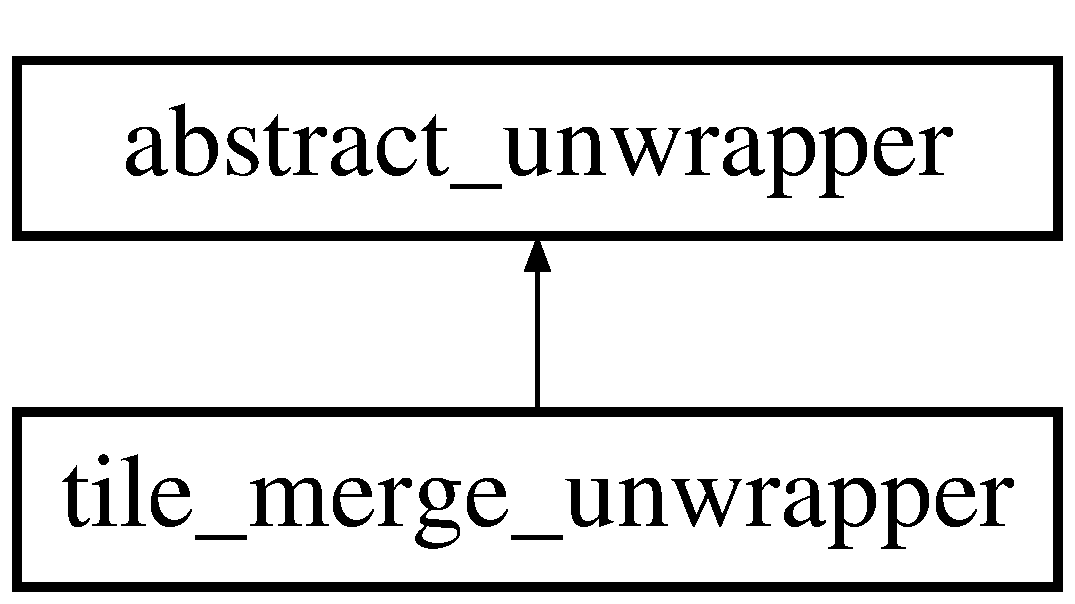
\includegraphics[height=2.000000cm]{classtile__merge__unwrapper}
\end{center}
\end{figure}
\subsection*{Public Member Functions}
\begin{DoxyCompactItemize}
\item 
\hyperlink{classtile__merge__unwrapper_ab070881e616ad7e72398aa6d019ea60e}{tile\-\_\-merge\-\_\-unwrapper} (int N\-\_\-width\-\_\-hint, int N\-\_\-height\-\_\-hint, \hyperlink{classabstract__tile__unwrapper}{abstract\-\_\-tile\-\_\-unwrapper} $\ast$unwrapper, \hyperlink{classabstract__tile__merger}{abstract\-\_\-tile\-\_\-merger} $\ast$merger)
\item 
virtual bool \hyperlink{classtile__merge__unwrapper_a30e5ac52c9edcd0356a37565fd955f6f}{unwrap} (\hyperlink{classfloat__image}{float\-\_\-image} $\ast$wrapped\-\_\-phase\-\_\-image, \hyperlink{classfloat__image}{float\-\_\-image} $\ast$unwrapped\-\_\-phase\-\_\-image)
\end{DoxyCompactItemize}


\subsection{Detailed Description}
provides a comfortable way of handling the tile unwrapping and merging process to unwrap an image. The class is provides with an instant of an \hyperlink{classabstract__tile__unwrapper}{abstract\-\_\-tile\-\_\-unwrapper} and an \hyperlink{classabstract__tile__merger}{abstract\-\_\-tile\-\_\-merger} and will unwrap a given image using the two elements. The tiles will be first unwrapped individually using the tile\-\_\-unwrapper and then merged using the specified merger. 

\subsection{Constructor \& Destructor Documentation}
\hypertarget{classtile__merge__unwrapper_ab070881e616ad7e72398aa6d019ea60e}{\index{tile\-\_\-merge\-\_\-unwrapper@{tile\-\_\-merge\-\_\-unwrapper}!tile\-\_\-merge\-\_\-unwrapper@{tile\-\_\-merge\-\_\-unwrapper}}
\index{tile\-\_\-merge\-\_\-unwrapper@{tile\-\_\-merge\-\_\-unwrapper}!tile_merge_unwrapper@{tile\-\_\-merge\-\_\-unwrapper}}
\subsubsection[{tile\-\_\-merge\-\_\-unwrapper}]{\setlength{\rightskip}{0pt plus 5cm}tile\-\_\-merge\-\_\-unwrapper\-::tile\-\_\-merge\-\_\-unwrapper (
\begin{DoxyParamCaption}
\item[{int}]{N\-\_\-width\-\_\-hint, }
\item[{int}]{N\-\_\-height\-\_\-hint, }
\item[{{\bf abstract\-\_\-tile\-\_\-unwrapper} $\ast$}]{unwrapper, }
\item[{{\bf abstract\-\_\-tile\-\_\-merger} $\ast$}]{merger}
\end{DoxyParamCaption}
)}}\label{classtile__merge__unwrapper_ab070881e616ad7e72398aa6d019ea60e}
Initialize the unwrapper. 
\begin{DoxyParams}{Parameters}
{\em tile\-\_\-\-N\-\_\-width\-\_\-hint} & Number of tiles in width direction. The actual number used will be close but is probably not identical (see \hyperlink{classtesselated__image}{tesselated\-\_\-image}). \\
\hline
{\em tile\-\_\-\-N\-\_\-height\-\_\-hint} & Number of tiles in height direction. The actual number used will be close but is probably not identical (see \hyperlink{classtesselated__image}{tesselated\-\_\-image}). \\
\hline
{\em unwrapper} & This unwrapper will perform the unwrap process of the individual tiles. \\
\hline
{\em merger} & This is the merger that merges the unwrapped tiles. \\
\hline
\end{DoxyParams}


\subsection{Member Function Documentation}
\hypertarget{classtile__merge__unwrapper_a30e5ac52c9edcd0356a37565fd955f6f}{\index{tile\-\_\-merge\-\_\-unwrapper@{tile\-\_\-merge\-\_\-unwrapper}!unwrap@{unwrap}}
\index{unwrap@{unwrap}!tile_merge_unwrapper@{tile\-\_\-merge\-\_\-unwrapper}}
\subsubsection[{unwrap}]{\setlength{\rightskip}{0pt plus 5cm}bool tile\-\_\-merge\-\_\-unwrapper\-::unwrap (
\begin{DoxyParamCaption}
\item[{{\bf float\-\_\-image} $\ast$}]{wrapped\-\_\-phase\-\_\-image, }
\item[{{\bf float\-\_\-image} $\ast$}]{unwrapped\-\_\-phase\-\_\-image}
\end{DoxyParamCaption}
)\hspace{0.3cm}{\ttfamily [virtual]}}}\label{classtile__merge__unwrapper_a30e5ac52c9edcd0356a37565fd955f6f}
This object will copy the input image since the tile-\/based unwrap procedures will alternate the input image. 
\begin{DoxyParams}{Parameters}
{\em wrapped\-\_\-phase\-\_\-image} & \\
\hline
{\em unwrapped\-\_\-phase\-\_\-image} & \\
\hline
\end{DoxyParams}
\begin{DoxyReturn}{Returns}

\end{DoxyReturn}


Implements \hyperlink{classabstract__unwrapper_a6d5c72cae9fcea45668cb02ddd3d9012}{abstract\-\_\-unwrapper}.



The documentation for this class was generated from the following files\-:\begin{DoxyCompactItemize}
\item 
include/block\-\_\-srncp/tile\-\_\-merge\-\_\-unwrapper.\-h\item 
src/block\-\_\-srncp/tile\-\_\-merge\-\_\-unwrapper.\-cpp\end{DoxyCompactItemize}

\hypertarget{classtilegroup}{\section{tilegroup Class Reference}
\label{classtilegroup}\index{tilegroup@{tilegroup}}
}
\subsection*{Public Member Functions}
\begin{DoxyCompactItemize}
\item 
\hyperlink{classtilegroup_aa6c6f357f5ff2da2c609ec88695256dc}{$\sim$tilegroup} ()
\begin{DoxyCompactList}\small\item\em Destruktor. \end{DoxyCompactList}\item 
void \hyperlink{classtilegroup_a4bec8ed94afb7cf220641232f86e92eb}{add\-\_\-tile} (\hyperlink{classtile}{tile} $\ast$t)
\item 
int \hyperlink{classtilegroup_a77326f80d6ec031a7429f574591cc3ee}{size} ()
\item 
void \hyperlink{classtilegroup_a2c453918b11a2bc1f0cd5f8f7746a5b7}{add\-\_\-value} (float val)
\end{DoxyCompactItemize}
\subsection*{Static Public Member Functions}
\begin{DoxyCompactItemize}
\item 
static \hyperlink{classtilegroup}{tilegroup} $\ast$ \hyperlink{classtilegroup_a1f6b1c44202332fa7271bae39e30981d}{create\-\_\-new} ()
\end{DoxyCompactItemize}
\subsection*{Friends}
\begin{DoxyCompactItemize}
\item 
void \hyperlink{classtilegroup_ae067cbd35e55edd62f9eb0158d925a21}{merge\-\_\-tilegroups} (\hyperlink{classtilegroup}{tilegroup} $\ast$g1, \hyperlink{classtilegroup}{tilegroup} $\ast$g2)
\end{DoxyCompactItemize}


\subsection{Detailed Description}
a helper class that groups tiles into a single group It allows easy access to all elements of a tile group. 

\subsection{Constructor \& Destructor Documentation}
\hypertarget{classtilegroup_aa6c6f357f5ff2da2c609ec88695256dc}{\index{tilegroup@{tilegroup}!$\sim$tilegroup@{$\sim$tilegroup}}
\index{$\sim$tilegroup@{$\sim$tilegroup}!tilegroup@{tilegroup}}
\subsubsection[{$\sim$tilegroup}]{\setlength{\rightskip}{0pt plus 5cm}tilegroup\-::$\sim$tilegroup (
\begin{DoxyParamCaption}
{}
\end{DoxyParamCaption}
)}}\label{classtilegroup_aa6c6f357f5ff2da2c609ec88695256dc}


Destruktor. 

S\-E\-G\-F\-A\-U\-L\-T?

\href{http://stackoverflow.com/questions/10464992/c-delete-vector-objects-free-memory}{\tt http\-://stackoverflow.\-com/questions/10464992/c-\/delete-\/vector-\/objects-\/free-\/memory} 

\subsection{Member Function Documentation}
\hypertarget{classtilegroup_a4bec8ed94afb7cf220641232f86e92eb}{\index{tilegroup@{tilegroup}!add\-\_\-tile@{add\-\_\-tile}}
\index{add\-\_\-tile@{add\-\_\-tile}!tilegroup@{tilegroup}}
\subsubsection[{add\-\_\-tile}]{\setlength{\rightskip}{0pt plus 5cm}void tilegroup\-::add\-\_\-tile (
\begin{DoxyParamCaption}
\item[{{\bf tile} $\ast$}]{t}
\end{DoxyParamCaption}
)}}\label{classtilegroup_a4bec8ed94afb7cf220641232f86e92eb}
Add an Element to this group. The pointer to the tilegroup is updated in for the given tile t and O\-N\-L\-Y F\-O\-R T\-H\-I\-S T\-I\-L\-E and not any other tiles in any other group it might have been in. 
\begin{DoxyParams}{Parameters}
{\em t} & Tile to add to this group. \\
\hline
\end{DoxyParams}
\hypertarget{classtilegroup_a2c453918b11a2bc1f0cd5f8f7746a5b7}{\index{tilegroup@{tilegroup}!add\-\_\-value@{add\-\_\-value}}
\index{add\-\_\-value@{add\-\_\-value}!tilegroup@{tilegroup}}
\subsubsection[{add\-\_\-value}]{\setlength{\rightskip}{0pt plus 5cm}void tilegroup\-::add\-\_\-value (
\begin{DoxyParamCaption}
\item[{float}]{val}
\end{DoxyParamCaption}
)}}\label{classtilegroup_a2c453918b11a2bc1f0cd5f8f7746a5b7}
Add value to all tiles. 
\begin{DoxyParams}{Parameters}
{\em val} & The value to add. \\
\hline
\end{DoxyParams}
\hypertarget{classtilegroup_a1f6b1c44202332fa7271bae39e30981d}{\index{tilegroup@{tilegroup}!create\-\_\-new@{create\-\_\-new}}
\index{create\-\_\-new@{create\-\_\-new}!tilegroup@{tilegroup}}
\subsubsection[{create\-\_\-new}]{\setlength{\rightskip}{0pt plus 5cm}static {\bf tilegroup}$\ast$ tilegroup\-::create\-\_\-new (
\begin{DoxyParamCaption}
{}
\end{DoxyParamCaption}
)\hspace{0.3cm}{\ttfamily [inline]}, {\ttfamily [static]}}}\label{classtilegroup_a1f6b1c44202332fa7271bae39e30981d}
Creates a new tilegroup. This is so new groups can only be created on the heap; \begin{DoxyReturn}{Returns}

\end{DoxyReturn}
\hypertarget{classtilegroup_a77326f80d6ec031a7429f574591cc3ee}{\index{tilegroup@{tilegroup}!size@{size}}
\index{size@{size}!tilegroup@{tilegroup}}
\subsubsection[{size}]{\setlength{\rightskip}{0pt plus 5cm}int tilegroup\-::size (
\begin{DoxyParamCaption}
{}
\end{DoxyParamCaption}
)}}\label{classtilegroup_a77326f80d6ec031a7429f574591cc3ee}
\begin{DoxyReturn}{Returns}
The number of elements in the tilegroup. 
\end{DoxyReturn}


\subsection{Friends And Related Function Documentation}
\hypertarget{classtilegroup_ae067cbd35e55edd62f9eb0158d925a21}{\index{tilegroup@{tilegroup}!merge\-\_\-tilegroups@{merge\-\_\-tilegroups}}
\index{merge\-\_\-tilegroups@{merge\-\_\-tilegroups}!tilegroup@{tilegroup}}
\subsubsection[{merge\-\_\-tilegroups}]{\setlength{\rightskip}{0pt plus 5cm}void merge\-\_\-tilegroups (
\begin{DoxyParamCaption}
\item[{{\bf tilegroup} $\ast$}]{g1, }
\item[{{\bf tilegroup} $\ast$}]{g2}
\end{DoxyParamCaption}
)\hspace{0.3cm}{\ttfamily [friend]}}}\label{classtilegroup_ae067cbd35e55edd62f9eb0158d925a21}
Merges the tiles from 2 groups into one group. Group g2 is merged into g1. 
\begin{DoxyParams}{Parameters}
{\em g1} & First group \\
\hline
{\em g2} & Second group. \\
\hline
\end{DoxyParams}


The documentation for this class was generated from the following files\-:\begin{DoxyCompactItemize}
\item 
include/block\-\_\-srncp/tile.\-h\item 
src/block\-\_\-srncp/tilegroup.\-cpp\end{DoxyCompactItemize}

\input{class_ui__digiholo_main_gui}
%--- End generated contents ---

% Index
\newpage
\phantomsection
\addcontentsline{toc}{chapter}{Index}
\printindex

\end{document}
